%% ----------------------------------------------------------------
%% Thesis.tex -- MAIN FILE (the one that you compile with LaTeX)
%% ---------------------------------------------------------------- 

% Set up the document
\documentclass[a4paper, 11pt, oneside]{Thesis}  % Use the "Thesis" style, based on the ECS Thesis style by Steve Gunn
\graphicspath{Figures/}  % Location of the graphics files (set up for graphics to be in PDF format)

% Include any extra LaTeX packages required
\usepackage[square, numbers, comma, sort&compress]{natbib}  % Use the "Natbib" style for the references in the Bibliography
\usepackage{verbatim}  % Needed for the "comment" environment to make LaTeX comments
\usepackage{vector}  % Allows "\bvec{}" and "\buvec{}" for "blackboard" style bold vectors in maths
\hypersetup{urlcolor=cyan, colorlinks=true, linktocpage=true}  % Colours hyperlinks in blue, but this can be distracting if there are many links.


%%%%%% Start: Kelvin's Packages %%%%%% 
\usepackage{placeins}
\usepackage{wrapfig}
\usepackage[noabbrev]{cleveref}
\usepackage[usenames,dvipsnames]{xcolor}
\bibliographystyle{unsrtnat}
%\usepackage[apaciteclassic]{apacite}
%\bibliographystyle{apacite}
%%%%%% End: Kelvin's Packages %%%%%% 


%%%%%% Start: Kelvin's Macro's %%%%%% 

\newcommand{\includefigure}[4]
{
	\begin{figure}[!htbp]
		\centering
			\includegraphics[width=#4\textwidth]{Figures/#1.#2}
		\caption{#3}
		\label{Figure:#1}
	\end{figure}
	
	\FloatBarrier
}

\newcommand{\matern}{Mat\'{e}rn }
\newcommand{\maternmath}{Mat\acute{e}rn }
\renewcommand{\vec}[1]{\boldsymbol{#1}}

%%%%%% End: Kelvin's Macro's %%%%%% 
%% ----------------------------------------------------------------
\begin{document}
\frontmatter      % Begin Roman style (i, ii, iii, iv...) page numbering

% Set up the Title Page
\title  {Honours Thesis \\ \textnormal{Informative Path Planning with Gaussian Process Classifiers for Seafloor Exploration}}
\authors  {\texorpdfstring
            {\href{yhsu9975@uni.sydney.edu.au}{Yuan-Shuo Kelvin Hsu}}
            {Yuan-Shuo Kelvin Hsu}
            }
\addresses  {\groupname\\\deptname\\\univname}  % Do not change this here, instead these must be set in the "Thesis.cls" file, please look through it instead
\date       {\today}
\subject    {}
\keywords   {}

\maketitle
%% ----------------------------------------------------------------

\setstretch{1.3}  % It is better to have smaller font and larger line spacing than the other way round

% Define the page headers using the FancyHdr package and set up for one-sided printing
\fancyhead{}  % Clears all page headers and footers
\rhead{\thepage}  % Sets the right side header to show the page number
\lhead{}  % Clears the left side page header

\pagestyle{fancy}  % Finally, use the "fancy" page style to implement the FancyHdr headers

%% ----------------------------------------------------------------
% Declaration Page required for the Thesis, your institution may give you a different text to place here
\Declaration{

\addtocontents{toc}{\vspace{1em}}  % Add a gap in the Contents, for aesthetics

I, Yuan-Shuo Kelvin Hsu, declare that this thesis titled, `Informative Path Planning with Gaussian Process Classifiers for Seafloor Exploration' and the work presented in it are my own. I confirm that:

\begin{itemize} 
\item[\tiny{$\blacksquare$}] This work was done wholly or mainly while in candidature for a research degree at this University.
 
\item[\tiny{$\blacksquare$}] Where any part of this thesis has previously been submitted for a degree or any other qualification at this University or any other institution, this has been clearly stated.
 
\item[\tiny{$\blacksquare$}] Where I have consulted the published work of others, this is always clearly attributed.
 
\item[\tiny{$\blacksquare$}] Where I have quoted from the work of others, the source is always given. With the exception of such quotations, this thesis is entirely my own work.
 
\item[\tiny{$\blacksquare$}] I have acknowledged all main sources of help.
 
\item[\tiny{$\blacksquare$}] Where the thesis is based on work done by myself jointly with others, I have made clear exactly what was done by others and what I have contributed myself.
\\
\end{itemize}
 
 
Signed:\\
\rule[1em]{25em}{0.5pt}  % This prints a line for the signature
 
Date:\\
\rule[1em]{25em}{0.5pt}  % This prints a line to write the date
}
\clearpage  % Declaration ended, now start a new page

%% ----------------------------------------------------------------
% The "Funny Quote Page"
\pagestyle{empty}  % No headers or footers for the following pages

\null\vfill
% Now comes the "Funny Quote", written in italics
%\textit{``Write a funny quote here.''}
%
%\begin{flushright}
%If the quote is taken from someone, their name goes here
%\end{flushright}

\vfill\vfill\vfill\vfill\vfill\vfill\null
\clearpage  % Funny Quote page ended, start a new page
%% ----------------------------------------------------------------

% The Abstract Page
\addtotoc{Abstract}  % Add the "Abstract" page entry to the Contents
\abstract{
\addtocontents{toc}{\vspace{1em}}  % Add a gap in the Contents, for aesthetics
	
	While underwater terrains have been mapped extensively over the last century, geological and ecology studies of marine environments only began in recent years. Unlike ocean terrain mapping, collection of marine environment data and imagery requires \textit{in situ} exploration, and is significantly slower and costly. This thesis investigates machine learning methods for autonomous underwater vehicles to intelligently and actively plan an underwater path for data collection. The problem is complicated by the presence of dynamic uncertainties that is highly dependent on the vehicle's planning actions. A dynamic planning method is proposed to maximise information gained, or minimise overall entropy, in a given underwater region, while constrained by cost and time.
}

\clearpage  % Abstract ended, start a new page
%% ----------------------------------------------------------------

\setstretch{1.3}  % Reset the line-spacing to 1.3 for body text (if it has changed)

% The Acknowledgements page, for thanking everyone
%\acknowledgements{
%\addtocontents{toc}{\vspace{1em}}  % Add a gap in the Contents, for aesthetics
%
%The acknowledgements and the people to thank go here, don't forget to include your project advisor\ldots
%
%}
\clearpage  % End of the Acknowledgements
%% ----------------------------------------------------------------

\pagestyle{fancy}  %The page style headers have been "empty" all this time, now use the "fancy" headers as defined before to bring them back

%% ----------------------------------------------------------------
\lhead{\emph{Contents}}  % Set the left side page header to "Contents"
\tableofcontents  % Write out the Table of Contents

%% ----------------------------------------------------------------
\lhead{\emph{List of Figures}}  % Set the left side page header to "List if Figures"
\listoffigures  % Write out the List of Figures

%% ----------------------------------------------------------------
\lhead{\emph{List of Tables}}  % Set the left side page header to "List of Tables"
\listoftables  % Write out the List of Tables

%% ----------------------------------------------------------------
\setstretch{1.5}  % Set the line spacing to 1.5, this makes the following tables easier to read
\clearpage  % Start a new page
\lhead{\emph{Abbreviations}}  % Set the left side page header to "Abbreviations"
\listofsymbols{ll}  % Include a list of Abbreviations (a table of two columns)
{
% \textbf{Acronym} & \textbf{W}hat (it) \textbf{S}tands \textbf{F}or \\
		ACFR & Australian Centre of Field Robotics \\
		API & Application Programming Interface \\
		AUV & Autonomous Underwater Vehicle \\
		AVA & All v.s. All \\
		\\
		BDKD & Big Data Knowledge Discovery \\
		BO & Bayesian Optimisation \\
		\\
		CDF & Cumulative Distribution Function \\
		\\
		EP & Expectation Propagation \\
		\\
		iid & independent and identically distributed \\
		\\
		GP & Gaussian Process \\ 
		GPBC & Gaussian Process Binary Classification \\
		GPC & Gaussian Process Classification \\
		GPLSC & Gaussian Process Least Squares Classifier \\
		GPMC & Gaussian Process Multi-Class Classification \\
		GPR & Gaussian Process Regression \\
		\\
		LE & Linearised Entropy \\
		LIDAR & Light Detection And Ranging \\
		LP & Laplace Approximation \\
		\\
		MCJE & Monte Carlo Joint Entropy \\
		MDP & Markov Decision Processes \\
		\\
		NICTA & National ICT Australia \\
		\\
		OVA & One v.s. All \\
		\\
		P1NN & Probabilistic One Nearest Neighbor \\
		PDF & Probability Distribution Function \\
		PLS & Probabilistic Least Squares \\
		POMDP & Partially Observable Markov Decision Processes \\
		PRM	& Probabilistic Road Map \\
		\\
		SBO & Sequantial Bayesian Optimisation \\
		SE & Squared Exponential \\
		SIEF & Science \& Industry Endowment Fund \\
		SONAR & Sound Navigation And Ranging \\
}

%% ----------------------------------------------------------------
\clearpage  % Start a new page
\lhead{\emph{Physical Constants}}  % Set the left side page header to "Physical Constants"
\listofconstants{lrcl}  % Include a list of Physical Constants (a four column table)
{
%	% Constant Name & Symbol & = & Constant Value (with units) \\
%	Speed of Light & $c$ & $=$ & $2.997\ 924\ 58\times10^{8}\ \mbox{ms}^{-\mbox{s}}$ (exact)\\

}

%% ----------------------------------------------------------------
\clearpage  %Start a new page
\lhead{\emph{Symbols}}  % Set the left side page header to "Symbols"
\listofnomenclature{lll}  % Include a list of Symbols (a three column table)
{
%	% symbol & name & unit \\
%	$a$ & distance & m \\
%	$P$ & power & W (Js$^{-1}$) \\
%	& & \\ % Gap to separate the Roman symbols from the Greek
%	$\omega$ & angular frequency & rads$^{-1}$ \\
}
%% ----------------------------------------------------------------
% End of the pre-able, contents and lists of things
% Begin the Dedication page


\lhead{Active Path Planning for Ocean Terrain Exploration}
\setstretch{1.3}  % Return the line spacing back to 1.3

%\pagestyle{empty}  % Page style needs to be empty for this page
%\dedicatory{For/Dedicated to/To my\ldots}

\addtocontents{toc}{\vspace{2em}}  % Add a gap in the Contents, for aesthetics


%% ----------------------------------------------------------------
\mainmatter	  % Begin normal, numeric (1,2,3...) page numbering
\pagestyle{fancy}  % Return the page headers back to the "fancy" style

% Include the chapters of the thesis, as separate files
% Just uncomment the lines as you write the chapters

\chapter{Introduction}
\lhead{Introduction}
\label{Introduction}

	\section{Motivation}
	\label{Introduction:Motivation}
	
		Thanks to optical and acoustic depth sounding technology, detailed ocean terrain maps across a majority of the globe have become increasingly accessible. These information generally takes the form of \textit{Bathymetric} data - recordings of measured depth, slope, roughness, and similar structural information that summarises the seafloor topography. Currently, bathymetric data has been recorded with advanced techniques such as SONAR (\textbf{SO}und \textbf{N}avigation \textbf{A}nd \textbf{R}anging), LIDAR (\textbf{LI}ght \textbf{D}etection \textbf{A}nd \textbf{R}anging), and Multibeam Echosounder for more than half a century \citep{Niedzielski2013231, Colbo201441}. With such volume of bathymetric information, we can reconstruct accurate 3D models for the seafloor terrain through spatial analytics and modeling techniques \citep{Niedzielski2013231}.
		
		However, bathymetric data only contains information regarding the spatial structure of the marine terrain. It provides no indication towards the types of marine habitats that resides within parts of the ocean, nor does it contain clues regarding the minerals or natural resources that may be present. Today, less than five percent of seafloor habitats have been explored \citep{NOAA}. As the ocean covers more than 70\% of the globe, this leaves more than 67\% of the planet's habitats unexplored despite our deep reliance on much of these undiscovered ecosystems. With big data analysis becoming more feasible in recent years, there has been an increase in scientific and economical demands - from ecologist and geologists to resource and mining industries - for the ability to predict or infer the types of marine habitats or natural resources residing at various marine environments.
		
		Thus, unlike the case for bathymetric data, there is currently a lack of \textit{label} data, which is a summary of the habitats, resources, and other interesting properties observed at various parts of the ocean. This implies the need to map the ocean floor again for label data using vision based sensing equipments. In order to understand the ecological, geological, chemical, and archaeological aspects of the ocean floor, autonomous underwater vehicles (AUVs) are now capable of efficiently collecting information and observations from natural environments of large spatial scale. In the case of benthic habitat mapping, AUVs collect imagery data of seafloor environments, which are then associated with a particular \textit{label} with semantic meaning \citep{Steinberg2015128}. For example, imageries of `coral' regions receive the label `coral'. Unfortunately, while bathymetric data can often be measured with decent accuracy at a distance (for example, with SONAR from ships at sea level), such visual imagery can only be obtained through expensive AUV missions that travel deep into the ocean to image underwater environments at a close distance. Together with the immense spatial scale of the benthic seafloor to be explored, this implies that it is impractical to map exhaustively the entire region of interest (ROI) under any reasonable time and cost. Furthermore, AUV missions are limited by power supply, data storage, and computational capabilities \citep{AsherBender}, further limiting the time and hence coverage each AUV mission can achieve. 
		
		As such, AUVs must prioritise exploring sub-domains of the ROI that ideally contain the most important and valuable information. This is a form of spatial sampling problem \citep{Rigby:ROB20372}, which aims to address the question: given the choice to observe only a few parts of the region of interest, how should one infer the best candidates for observation? AUV missions add another layer of complication to the spatial sampling problem - the candidate locations must form continuous paths that the AUV can physically travel.
		
		This is known as the \textit{informative path planning problem}. The objective of informative path planning is to minimise the overall uncertainty regarding the entire region of interest by traversing the most informative path.
		
		This thesis addresses the informative path planning problem for benthic habitat mapping. There are two main aspects to informative seafloor exploration for which this thesis is concerned with. The first part of this thesis is focused on benthic habitat mapping, where techniques of habitat classification and inference are discussed. The basic theory under which information and uncertainty are measured and quantified are developed and formulated in the general framework, which is then applied to benthic habitat mapping. The second part of this thesis then proceeds to investigate the informative seafloor exploration problem. Using the properties of inference models developed for benthic habitat mapping, a range of path planning policies are discussed and compared. Practical considerations of computational tractability and flexibility then lead to compromises between optimality and feasibility. Finally, this thesis proposes a practical framework for AUVs to autonomously plan informative paths that achieves the highest mapping rate under a classification accuracy criterion.
		
	\section{Objectives}
	\label{Introduction:Objective}
		The high level objective of this thesis is to develop an informative seafloor exploration policy that can produce benthic habitat maps efficiently. Specifically, this thesis focuses on the theoretical and computational aspects of informative path planning that is practical for seafloor mapping. The aim is to address the informative seafloor exploration problem in a principled manner with theoretical grounding, while taking computational feasibility into account. 
		
		The goal of this thesis can be summarised as follows:
		
		\begin{quote}
			To investigate informative seafloor exploration policies for an AUV with limited mission time, in order to map benthic habitats faster in a principled and computationally feasible way.
		\end{quote}
%	
%		The high level objective of this thesis is to develop and design an underwater path planner such that the resulting path minimises the overall mapping error of the seafloor region of interest.
%		
%		Detailed examination of this objective would raise details that would need to be made more specific.
%		
%		Firstly, the measure of entropy would be highly dependent on the quantities or qualities the vehicle is to search for, as well as the underwater region of interest. It would need to be examined to ensure that it is an appropriate measure of the environment uncertainty to be reduced that is relevant to the mission.
%		
%		Secondly, finding paths that subsequently minimises the overall entropy is fundamentally a dynamic programming and optimisation problem. As with any optimisation problem, problem constraints are to be defined and made clear. Within the presence of possibly difficult dynamical constraints, it is likely that simplifications are necessary at various stages of the thesis.
%		
%		Another consideration is the feasibility of the algorithm. While it can be difficult to measure the optimality of any solution proposed, it is often easier to examine the feasibility of the algorithm through studying the hardware constraints involved or the physical environment. One of the most important feasibility constraint relevant to this thesis is the computational capabilities of the vehicle computer hardware. Depending on the final proposed algorithm, it may not always be possible for the path planer to be executed in a fully online fashion. A more likely situation would involve planning a path to be executed for a duration of time and update the path through re-planning at a frequency much lower than the vehicle is navigating. For short missions, it may be more desirable to have the entire path planned offline.
%		
%		Other subtleties arise from the nature of the the underwater path planning problem. There is often no goal location, only an objective to maximise the information gained. This is a form of active path planning, which is similar to the active sampling philosophy but with dynamic constraints.
%		
%		Finally, other than the path planning algorithm, a major part of this thesis revolves around modeling the ocean environment accurately. Without an accurate understanding of the ocean environment, the vehicle cannot plan a path that is of reasonable significance. This thesis is to address the ways the ocean environment is to be modeled, develop these algorithms, and implement them on an ocean exploration setting.
%		
%		The detailed objective of this thesis is thus to examine and address all the concerns above, and to provide a better understanding towards the methods these active path planning problems can be approached.
		
	\section{Contribution}
	\label{Introduction:Contribution}
	
		This thesis is concerned with mapping seafloor benthic habitats efficiently in a principled manner. Specific contributions and focuses of this thesis are:
		
		\begin{itemize}
		
			\item A computationally efficient, parallelisable implementation for multiclass Gaussian process (GP) classifiers through the One versus All (OVA) scheme. Time and spatial complexity of the classifier are further improved through taking advantage of the GP classifier structure. Under Laplace approximation, this approach avoids the computational complexity from Monte Carlo sampling that is required in the inference stage. The computational framework is consistent with sparsification techniques for further complexity improvement although this is not necessary.
			
			\item An All versus All (AVA) approach to GP multiclass classification. While OVA techniques have been employed in various settings in the literature, there is no direct treatment of GP multiclass classification using All versus All classifiers, which achieves predictions with less biases due to a more balanced binary comparison between classes \textit{under balanced data}. It also shares the above advantages with OVA classifiers. This provides another choice for GP multiclass classification apart from the OVA approach.

			\item Two new ways for probability fusion in the GP multiclass classification setting under the One versus All and All versus All approach - mode keeping and exclusion. For the All versus All case, techniques for pre-fusing the probabilities into an appropriate form is also investigated and derived. These methods provide better properties when used for compute entropy of predictions as compared to simple normalisation techniques.
			
			\item A Monte Carlo based method for estimating the joint prediction information entropy hereby named \textit{Monte Carlo Prediction Information Entropy} (MCPIE). This work aims to provide a framework to obtain the joint prediction information entropy that is traditionally missing the the treatment of Gaussian process classifiers. While there are no analytical forms for the joint prediction information entropy available, it can be shown that the Monte Carlo estimation converges in value under reasonable amounts of sample draws. A stable and efficient method for Monte Carlo Optimisation is also devised which allows MCPIE to be utilised with reasonable tractability in an information acquisition setting, hereby named \textit{MCPIE acquisition}.
			
			\item An alternative, analytically tractable entropy measure hereby named \textit{linearised model differential entropy} (LMDE). The LMDE of GP classifiers captures mutual information of a given region of interest. Specifically, instead of examining uncertainty with mainly prediction variance, LMDE also takes into account the prediction bias. Through addressing the bias-variance trade-off, a common challenge in machine learning algorithms, LMDE provides an alternative way to quantify uncertainty and information. Analytical tractability is then achieved through linearisation approximations. Linearised model differential entropy is proposed as an acquisition function for informative path planning, hereby referred to as \textit{LMDE acquisition}.
			
			\item A receding horizon framework to informative path planning. This provides a framework that is computationally efficient yet produce informative paths that are stable in performance. The main advantage of this approach is its low computational requirement in time and memory as it is not necessary to compute the acquisition criterion across the entire ROI as done in many informative seafloor exploration policies. Together with LMDE and MCPIE acquisition, the suitability of the receding horizon approach is demonstrated on the Scott Reef data set from \cite{IMOS}. This thesis demonstrates that under a receding horizon framework, LMDE and MCPIE acquisition achieves a faster mapping rate than other non-mutual, myopic, or non-informative approaches, and does so with reasonable computational resources. 
			
		\end{itemize}
			
	\section{Structure}
	\label{Introduction:Structure}
	
		The structure of this thesis is outlined as below.
		
%		Chapter \ref{Background} provides the necessary background and theory for the purpose of understanding this thesis. Related work in informative seafloor exploration are presented, as well as the various approaches that has been undertaken in this area. Most importantly, this chapter introduces and summarises the Gaussian process framework.
%		
%		Chapter \ref{BenthicHabitatMapping} details how the benthic habitat environment are modeled upon bathymetric features using Gaussian process classifiers. Most importantly, this chapter extends the usual Gaussian process classifier framework to multiclass classification that is not limited to Laplace approximation only. A general OVA and AVA framework for multiclass GP classification is developed, which is then applied to synthetic and real datasets to verify performance. These frameworks demand the use of probability fusion techniques in order to produce consistent inference and prediction results. The chapter concludes by applying the GP models developed to map the benthic habitat mapping at Scott Reef.
%		
%		Chapter \ref{InformativeSeafloorExploration} proceeds to focus on the theory and applications of informative path planning. The outset of this chapter begins by formulating a Monte Carlo approach for estimating the joint prediction information entropy of a prediction. The highlight of this chapter is the introduction and derivation of the linearised model differential entropy (LMDE) for both binary and multiclass GP classifiers. Comparisons with the usual prediction information entropy is presented to demonstrate their differences and respective advantages and disadvantages. This motivates the use of linearised model differential entropy as a suitable acquisition function for informative path planning. The discussion continues with a formulation of the receding horizon approach to informative path planning, and moves on to demonstrate the application of various acquisition criteria under this formulation. Description of the simulation experiment are provided, and properties of the approach observed from corresponding results are discussed and analysed. The performance of the proposed exploration policy are then assessed with a classification accuracy criterion.

		Chapter \ref{Background} provides the necessary background and theory for the purpose of understanding this thesis. After an introduction to the theory behind Bayesian modeling with Gaussian processes (section \ref{Background:GaussianProcesses}), a review of current literature in informative path planning quickly reveals the need for a more computationally efficient approach that is non-myopic while capturing mutual information (section \ref{Background:RelatedWork}).
		
		Chapter \ref{BenthicHabitatMapping} then begins by building upon the existing Gaussian process classification framework for benthic habitat mapping. The mapping problem is first formulated as a supervised learning problem which requires the habitat labels to be modeled upon appropriate bathymetric features (section \ref{BenthicHabitatMapping:BathymetricFeatures}). Through examining the binary classification framework, efficient and parallelisable multiclass classifiers in the OVA and AVA scheme are developed in a way that is not limited to Laplace approximation. These frameworks demand the use of probability fusion techniques in order to ensure consistent inference. As such, on top of simple normalisation, two novel probability fusion methods, mode keeping and exclusion, are devised which exhibit improved inference properties as demonstrated by illustrative test data (section \ref{BenthicHabitatMapping:Classification}). This chapter concludes by applying the GP classifiers developed to map the benthic habitats at Scott Reef, which sets up the initial scenario for informative exploration experiments (section \ref{BenthicHabitatMapping:ScottReef}).
		
		Chapter \ref{InformativeSeafloorExploration} moves on to investigate informative path planning techniques that build upon such Gaussian process classifiers. Through motivating the need for a measure of mutual information, a direct approach with Monte Carlo estimation is formulated in order to compute the \textit{joint} prediction information entropy, hereby named Monte Carlo prediction information entropy (MCPIE) (section \ref{InformativeSeafloorExploration:MCPIE}). Careful analysis of the predictive probabilities obtained under likelihood response transformations of the latent function then inspires the concept of model differential entropy (MDE). Analytical tractability is then achieved through a linearisation technique for the binary, multiclass OVA, and multiclass AVA scenario, thus producing the novel linearised model differential entropy (LMDE) mutual information measure (section \ref{InformativeSeafloorExploration:LMDE}). The two measures are compared in properties and performance, revealing their complementary nature which resembles the bias-variance trade-off that is ubiquitous in statistics and machine learning (section \ref{InformativeSeafloorExploration:ComparisonMutualEntropyMeasures}). A stable and efficient path planning scheme is then developed under the receding horizon formulation (section \ref{InformativeSeafloorExploration:RecedingHorizonFormulation}), where the implementation details that improve its tractability are outlined. The discussion proceeds to demonstrate the application of various acquisition criteria under this formulation. Description of the simulation experiment are provided, and properties of the approach observed from corresponding results are discussed and analysed. The performance of the proposed exploration policy are then assessed with a classification accuracy criterion, which reveals the effectiveness of MCPIE and especially LMDE acquisition approaches over alternative methods (section \ref{InformativeSeafloorExploration:ScottReef}).
				
		Finally, Chapter \ref{Conclusion} summarises the work presented in this thesis, the contributions made, and potentials for future improvements.

\chapter{Background}
\lhead{Background}
\label{Background}

	{\color{BurntOrange} Add Background Summary and Introduction}
	
	\section{Related Work}
	\label{Background:RelatedWork}
	
		One of the main challenges of informative path planning include selecting the appropriate acquisition function suitable for the type of exploration task at hand. \textit{Acquisition functions}, or \textit{acquisition criterion}, measures the desirability of observing a particular location. In the informative path planning scenario, the acquisition function evaluates the amount of total information or uncertainty contained by a given candidate path. In this context, the way in which \textit{total information} is quantified determines the acquisition function. The more information the path contains, the more desirable it is for the AUV to follow and take observations on that path. 

		The effectiveness of an acquisition function that measures mutual information throughout a particular given path has been thoroughly investigated in the literature \citep{AsherBender, Rigby:ROB20372, Krause:2008:NSP:1390681.1390689, Kapoor}. \textit{Mutual information} refers to a measure of information that takes into account the overlapping information within the region or path in consideration. In most spatial sampling contexts, it is unlikely that two given locations within a region or path are completely unrelated or uncorrelated. Observations in one location provides partial information regarding other locations, which is the primary reason that an accurate benthic habitat map can be obtained without visiting all locations within the region exhaustively. Without considering mutual information, an agent such as an AUV may be prompted to observe locations that contain similar information, thus achieving inefficient mapping.
		
		Several types of acquisition functions have been proposed in the benthic habitat mapping context. \cite{AsherBender} uses an acquisition criterion given by \eqref{Equation:AsherBenderAcquisitionCriterion} where $\pi^{m}_{i}$ is the probability of the habitat label being a member of class $m \in \{1, \dots, c\}$ at query location $i \in \{1, \dots, n^{\star}\}$. Here $c$ is the number of classes and $n^{\star}$ is the number of query points.
		
		\begin{equation}
			H = - \frac{1}{n^{\star}} \sum_{i = 1}^{n^{\star}} \sum_{m = 1}^{c} \pi^{m}_{i} \log(\pi^{m}_{i})
		\label{Equation:AsherBenderAcquisitionCriterion}
		\end{equation}
		
		For a given query point $i$, $- \sum_{m = 1}^{c} \pi^{m}_{i} \log(\pi^{m}_{i})$ is exactly the prediction information entropy (PIE) at location $i$, which captures the local model uncertainty and thus potential information. As a result, the acquisition criterion given in \eqref{Equation:AsherBenderAcquisitionCriterion} is the mean of the marginalised PIE across query points, which does not capture mutual information through considering the joint distributions of the class labels across multiple query points $i \in \{1, \dots, n^{\star}\}$. This acquisition criterion will be referred to as MPIE for mean of marginalised prediction information entropy. In this approach, the quality of the habitat models are assessed by utility functions that evaluate the confidence of the GP classifier prediction, which is the difference of the MPIE before and after an observation is made \eqref{Equation:AsherBenderMutualInformationCriterion} \citep{Rigby:ROB20372}. This utility is used in conjunction with a GP classifier under probabilistic least squares approximation to optimise selected survey paths through considering the differential entropy across the entire region of interest (ROI). Below, $X, \bvec{y}$ are the observed feature locations and habitat labels, $X^{\star}$ to be the unobserved query locations, and $X_{p}, \bvec{y}_{p}$ are the observations made after traversing the proposed path.
	
		\begin{equation}
			I = H[X^{\star} | X, \bvec{y}] - H[X^{\star} | X \cup X_{p}, \bvec{y} \cup \bvec{y}_{p}]
		\label{Equation:AsherBenderMutualInformationCriterion}
		\end{equation}
		
		\cite{Krause:2008:NSP:1390681.1390689} instead focuses on sensor placement methodologies to optimse mutual information gained. This aims to reduce predictive variance at all query points. The chosen acquisition function is the difference between the MIE at all \textit{final} unobserved locations $X^{\star} \backslash X_{p}$ before and after the observations are taken \eqref{Equation:KrauseAcquisitionCriterion}.
		
		\begin{equation}
			I = H[X^{\star} \backslash X_{p} | X, \bvec{y}] - H[X^{\star} \backslash X_{p} | X \cup X_{p}, \bvec{y} \cup \bvec{y}_{p}]
		\label{Equation:KrauseAcquisitionCriterion}
		\end{equation}
		
		Under the GP classification model, however, this results in an integral that can only be estimated through sampling techniques which are computationally expensive. As such, computationally tractable methods usually employ experimental design philosophies in minimising the predictive variance \citep{AsherBender}.
		
		\cite{Kapoor} demonstrates the use of posterior mean and covariance of the GP classifier latent function. While this approach takes full advantage of the analytical forms available for a Gaussian latent process, it does not consider the mutual behaviour of the unobserved locations with the proposed path.
		
		On the other hand, \cite{Roman:SequentialBayesianOptimisation} approaches the problem from a continuous path-planning perspective for UAVs in which two Gaussian processes are used - one to model the phenomenon and another to assess the quality of proposed paths. However, this layered Sequential Bayesian Optimisation approach is primarily devised for a regression setting which becomes intractable when performed in the classification domain.
		
		Much of the intractability discussed in such literature can trace its reason down to the fact that benthic habitat mapping is a classification problem instead of a regression problem. While Gaussian process regression provide analytical forms for inference, due to a non-Gaussian likelihood response, Gaussian process classification is no longer analytically tractable. Instead, several approximations must be made, which is discussed in section \ref{Background:GaussianProcesses:Classification}.
		
		This thesis addresses the tractability status of the problem through proposing an alternative acquisition criterion, hereby named linearised model differential entropy (LMDE), that captures mutual information. In the current literature, acquisition criterion either do not directly capture mutual information, such as \eqref{Equation:AsherBenderAcquisitionCriterion}, or take too long to compute due to required estimations from sampling, such as \eqref{Equation:KrauseAcquisitionCriterion}. This work shows that LMDE as an acquisition function captures an appropriate form of mutual information. Furthermore, LDME outperforms other acquisitions in both ractability and mapping accuracy.
		
	\section{Gaussian Processes}
	\label{Background:GaussianProcesses}
	
		Gaussian processes (GP) are stochastic processes which generalises the multi-variate Gaussian distribution. In a statistical learning and machine learning context, they are categorised as a type of \textit{supervised learning} method, which describes the problem of learning relationships between input and output variables from empirical data. The empirical data is also often referred to as the training set.
		
		Supervised learning methods are further categorised into regression and classification problems, depending on the nature of the output variable. The problem is a regression problem if the output is continuous, and a classification problem if the output is discrete. For example, when bathymetric feature extraction is analytically infeasible, bathymetric modeling becomes a regression problem, where the output variables are the bathymetric features. A common instance of the bathymetric modeling problem is seafloor depth modeling, in which the terrain elevation structure is the continuous output to be inferred. Benthic habitat mapping, on the other hand, involves inference of discrete habitat labels and is thus a classification problem.
		
		In both regression and classification settings, the input variables are often also referred to as \textit{features}, which motivated the term \textit{bathymetric features} in the previous sections. This also helps to distinguish the features from the spatial inputs, which are not necessarily the input variables involved in the supervised learning problem. In statistical literature, continuous regression outputs are sometimes called \textit{response} variables, although it is more often simply referred as the \textit{output} or \textit{target} in the machine learning community. However, in the Gaussian process classification setting, the term \textit{response} also refers to the likelihood response involved in the model. Therefore, the use of the term \textit{response} will be reserved for the latter in this thesis. Discrete classification outputs are often referred to as \textit{labels}, although the term \textit{target} is also used. In the benthic habitat mapping context, the type of henthic habitats are the labels to be inferred or predicted. 
		
		In the sections which references the use of Gaussian process models, $\bvec{x}$ will denote the input variable or features of the problem while $y$ will denote the output or target variable. Note that in general there are multiple features such that the input is a feature vector $\bvec{x}$. Without loss of generality, however, the output variable can always be treated as a scalar quantity $y$. Under cases of multiple output variables, the problem can be split into multiple single output variable problems.
		
		%%% If I need to talk about multi-task regressoin, put it in the appendix and put a note here saying that I can expand on this more.
		
		% It is true that prediction performance may be improved by considering the output vector together, which leads to multi-task regression, as will be briefly discussed. However, this is only the case if the training features the multiple outputs are located in different parts of the feature space, which does not occur for 

		The work presented here will be primarily based on \textit{Gaussian Process for Machine Learning} by \cite{GaussianProcessForMachineLearning}. 

		\subsection{Bayesian Modeling with Gaussian Processes}
		\label{Background:GaussianProcesses:BayesianModeling}
		
			The Gaussian process formulation follows the Bayesian modeling philosophy. An important distinction Bayesian modeling makes from the classical approach is the idea of estimating a distribution instead of a point value. While this is often more computationally expensive, it provides a very robust and accurate framework for prediction and inference. More importantly, it provides capabilities that classical approaches do not possess - the ability to quantify prediction uncertainties and, most importantly, potential information. 
			
			Suppose $H$ represents the event that a particular inference model $\mathcal{H}$ is representative of the true underlying phenomenon to be inferred. Further suppose $D$ represents the event that a particular set of observations $\mathcal{D}$ have been collected. The basic Bayesian modeling process begins with a \textit{prior} distribution $p(H)$, the probability of $\mathcal{H}$ being representative before $\mathcal{D}$ was observed, and updates this to a \textit{posterior} distribution $p(H | D)$, the updated probability of $\mathcal{H}$ being representative after observing $\mathcal{D}$. In this way, $\mathcal{H}$ can be interpreted as the agent's belief of the phenomenon. In the benthic habitat mapping context, the agent is the AUV, and the phenomenon is the type of benthic habitats distributed about the region of interest.
			
			In general, this belief update is achieved through Bayes theorem \eqref{Equation:Bayes}. The \textit{likelihood} distribution $p(D | H)$ is the probability of observing the dataset $\mathcal{D}$ given that $\mathcal{H}$ is representative of the true underlying phenomenon. The \textit{evidence} distribution $p(D)$ is the probability of observing the dataset. However, in practice it is often difficult to compute the evidence without a model. Hence, expanding over all possible inference models $\mathcal{H}$, the evidence can also be found by marginalising the joint distribution $p(D \cap H) = p(D | H) p(H)$ of observing $\mathcal{D}$ and $\mathcal{H}$ being representative \eqref{Equation:MarginalLikelihood}. In this way, the evidence is also referred to as the \textit{marginal likelihood}.
			
			\begin{equation}
				p(H | D) = \frac{p(D | H) p(H)}{p(D)} \qquad \Longleftrightarrow \qquad \mathrm{posterior} = \frac{\mathrm{likelihood} \times \mathrm{prior}}{\mathrm{evidence}}
			\label{Equation:Bayes}
			\end{equation}
			
			\begin{equation}
				p(D) = \sum_{H} p(D | H) p(H)
			\label{Equation:MarginalLikelihood}
			\end{equation}			
			
			This procedure is illustrated in \cref{Figure:BayesianModeling} for a Gaussian process with one dimensional input feature and output target. The mean prediction is shown as the black solid curve. Ten sample functions from the GP are drawn from the prior and posterior, represented by the coloured dashed curve. The shaded region represents the 2-$\sigma$ bounds of the prediction at each input feature value $x$. The prior distribution is updated to a posterior distribution after two points are observed. This example further serves to illustrate the concept of distributions over functions, which behaves as an infinite dimensional generalisation of a multivariate probability distribution. It is helpful to conceptualise functions as an infinite string of points, where functions can be interpreted as infinite dimensional vectors, such that drawing from an infinite dimensional distribution is equivalent to drawing from processes that operate on function space. Instead of drawing finite dimensional random vectors from distributions, a random function is drawn from a \textit{stochastic process} \footnote{When the input variable is temporal, a stochastic process can be more appropriately interpreted as having indefinite dimensional distributions.}.
			
			\begin{figure}[!htbp]
				\centering
					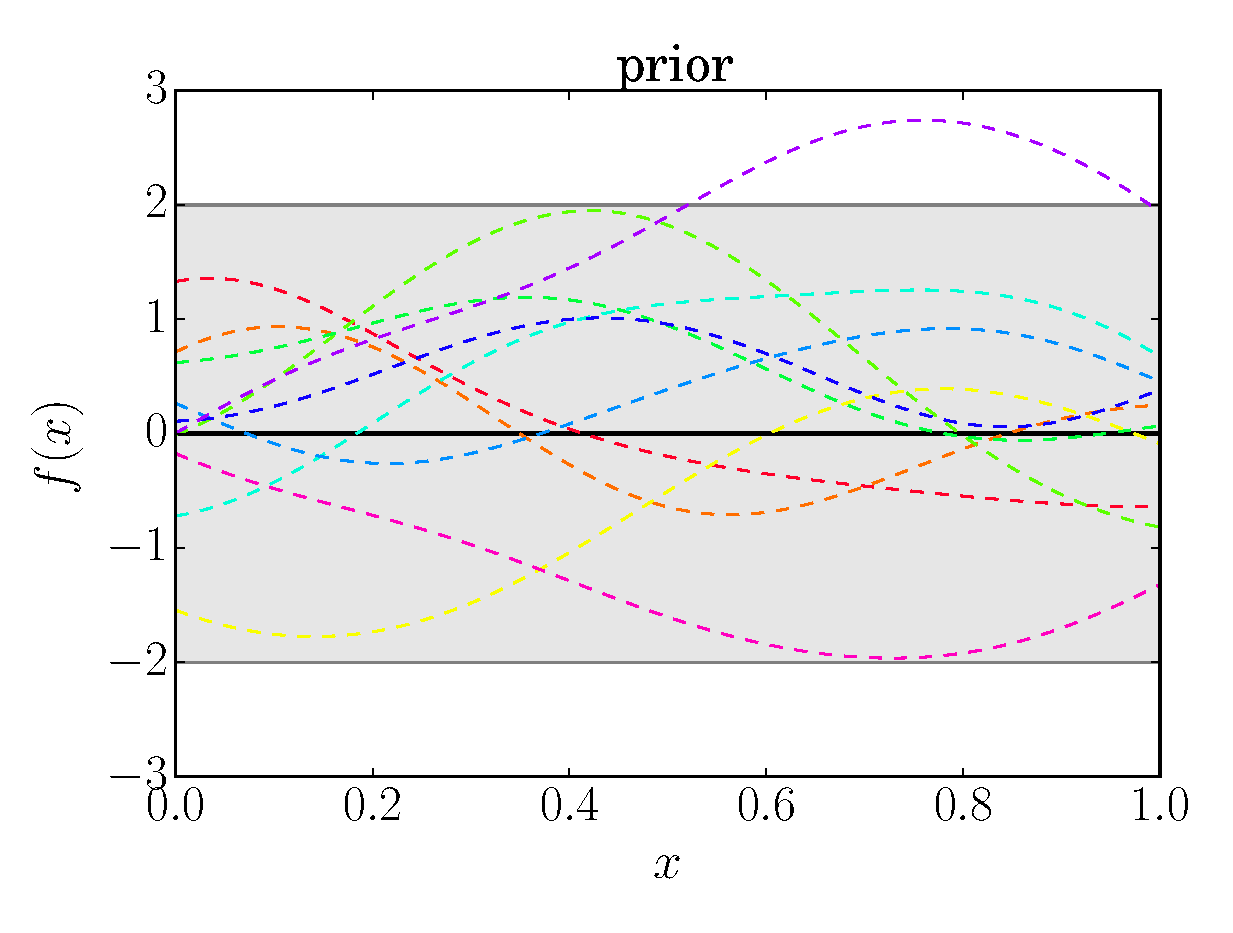
\includegraphics[width=0.48\textwidth]{Figures/bayesian_modeling/prior_draws.eps}
					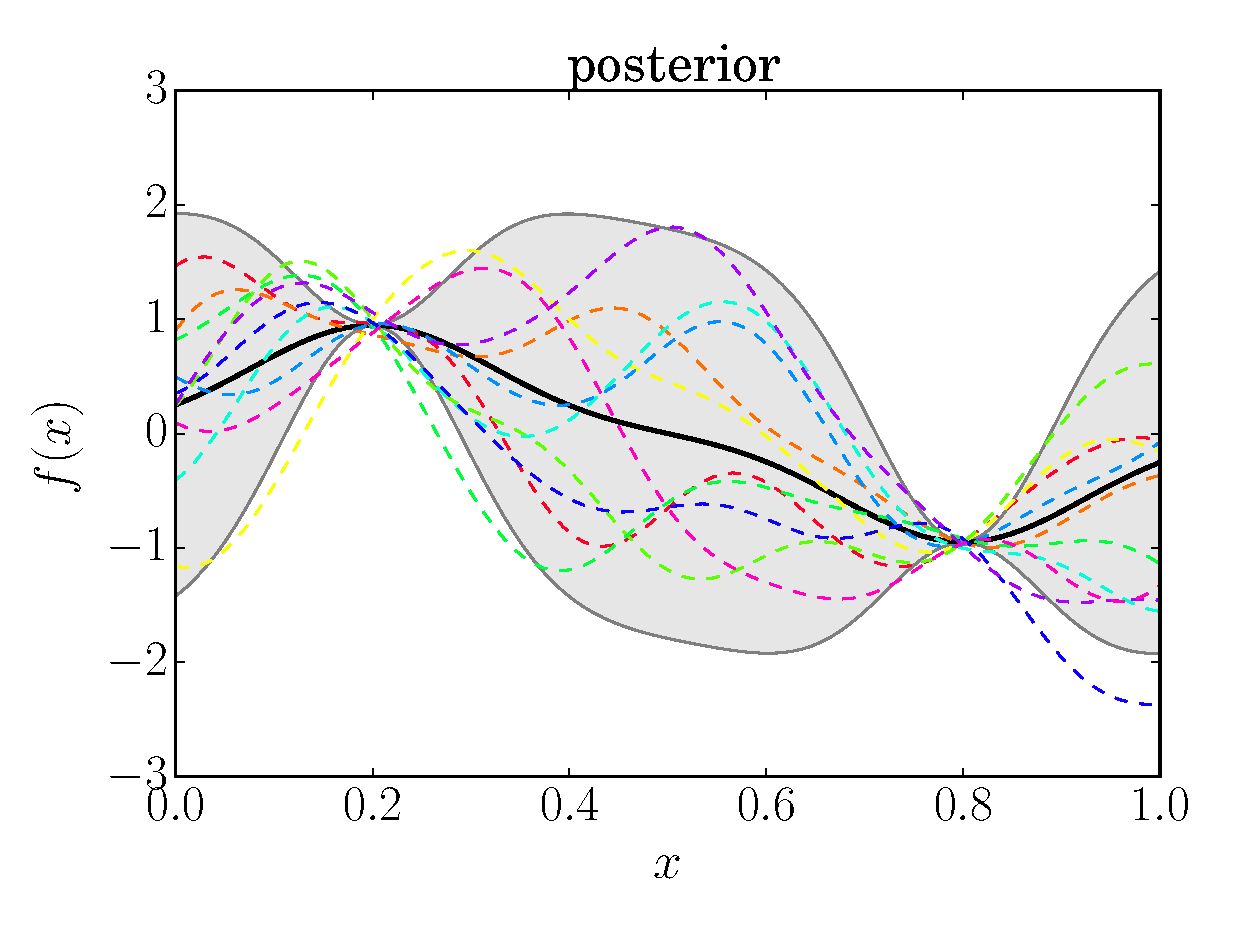
\includegraphics[width=0.48\textwidth]{Figures/bayesian_modeling/posterior_draws2.eps}
				\caption{Illustration of Gaussian Process Bayesian Modeling}
				\label{Figure:BayesianModeling}
			\end{figure}
			
			From this illustration, there are a few qualities one can notice. Firstly, the prior distribution is simply the zero function. The prior is meant to represent the system's current belief before the next observations are to be made. In this case, the prior situation involves no observations at all. Ideally, this means that the prior distribution should contain no predictive information. However, it is of philosophical note that all informative \footnote{It is certainly possible to perform inference without any assumptions. It will simply be uninformative in prediction or result.} inferences must begin with some assumptions regarding the structure of the phenomenon to be inferenced. In the illustration above, the function is assumed to be distributed as a process with zero mean. This assumption has excluded processes without means, such as the Cauchy process, as well as assumed a rather arbitrary mean function. However, this assumption is often valid as one can always pre-process the output data set through subtracting off their empirical mean so that the output is approximately distributed about zero. The representation of the standard deviation and hence variance as confidence bounds centred at the mean function also means that multi-model processes are excluded. For a Gaussian process, which is indeed uni-modal and have finite moments for all moments of finite degree, this illustration is common and useful for visualising the Bayesian modeling process. It is customary to visualise the 2-$\sigma$ bound for a Gaussian process. So, for this example, the prior distribution has a uniform standard deviation of one everywhere.
			
			Regarding the variance, a second observation is that the standard deviation and hence variance of the output function decreases at the observations, and gradually increases away from the observations. This leads to two remarks. Firstly, the variance or uncertainty of the output function at a location reduces when observations are made at that location. Secondly, neighboring points are related - the closer they are, the more related they are. This is seen through the observed points dragging nearby points towards it while reducing the uncertainty of nearby points. This resembles the concept of covariance. Evidently, points closer to each other have higher covariance then those further away, and the covariance beween the same points simply become its variance.
			
			The two observations above demonstrate that, just as a Gaussian distribution is defined through a mean vector and a covariance matrix, a Gaussian process is defined through a mean function $m(x)$ and a covariance function $k(x, x')$. In Gaussian process literature, the covariance function is also called a \textit{kernel} function.
			
			With an intuition of Gaussian processes in the Bayesian modeling context, a formal definition of Gaussian processes can now be introduced. In this thesis, the shorthand notation $I_{n} := \{1, 2, \dots, n\}$ will be used for concise indexing unless otherwise indicated, and is not to be confused with identity matrices $I_{p \times p} \in \mathbb{R}^{p \times p}$.
			
			\newpage
			\newtheorem{gpdef}{Gaussian Process}[section]
			\begin{gpdef}
				A random function $f(x)$, $x \in \mathbb{R}$, is distributed as a Gaussian process with mean function $m(x)$ and covariance function $k(x, x')$, if for any finite collection of feature points $\bvec{x} := [x_{1}, x_{2}, \dots, x_{n}]^{T}$, the corresponding output targets $\bvec{f}(\bvec{x}) := \{f(x_{i})\}_{i \in I_{n}} := [f(x_{1}), f(x_{2}), \dots, f(x_{n})]^{T}$ is jointly multivariate Gaussian distributed such that 

					\begin{equation}
						\bvec{f}(\bvec{x}) \sim \mathcal{N}(\bvec{m}(\bvec{x}), K(\bvec{x}, \bvec{x}'))
					\label{Equation:GaussianProcessFiniteDistribution}
					\end{equation}	
				
				where $\bvec{m}(\bvec{x}) :=  \{m(x_{i})\}_{i \in I_{n}} \in \mathbb{R}^{n}$ and $K(\bvec{x}, \bvec{x}') := \{k(x_{i}, x_{j})\}_{i \in I_{n}, j \in I_{n}}$. Such a function $f(x)$ is then notated as
				
					\begin{equation}
						f(x) \sim \mathcal{GP}(m(x), k(x, x'))
					\label{Equation:GaussianProcess}
					\end{equation}	
					
			\label{Definition:GaussianProcess}
			\end{gpdef}
			
			Certainly, this definition generalises finite dimensional multivariate Gaussian distributions, in that any subset of a multivariate Gaussian distributed random vector is also a multivariate Gaussian distributed of lower dimensionality.

			Definition \ref{Definition:GaussianProcess} is defined for a univariate input feature $x$. In fact, this definition generalises naturally to a multivariate input feature $\bvec{x} \in \mathbb{R}^{p}$ with $p$ features. This motivates definition \ref{Definition:GaussianRandomField}.
			
			\newtheorem{grfdef}{Gaussian Random Field}[section]
			\begin{grfdef}
				A random function $f(\bvec{x})$, $\bvec{x} \in \mathbb{R}^{p}$, is distributed as a Gaussian random field with mean function $m(\bvec{x})$ and covariance function $k(\bvec{x}, \bvec{x}')$, if for any finite collection of feature points $X := [\bvec{x}_{1}, \bvec{x}_{2}, \dots, \bvec{x}_{n}]^{T}$, the corresponding output targets $\bvec{f}(X) := \{f(\bvec{x}_{i})\}_{i \in I_{n}} := [f(\bvec{x}_{1}), f(\bvec{x}_{2}), \dots, f(\bvec{x}_{n})]^{T}$ is jointly multivariate Gaussian distributed such that 

					\begin{equation}
						\bvec{f}(X) \sim \mathcal{N}(\bvec{m}(X), K(X, X'))
					\label{Equation:GaussianRandomFieldFiniteDistribution}
					\end{equation}	
				
				where $\bvec{m}(X) :=  \{m(\bvec{x}_{i})\}_{i \in I_{n}} \in \mathbb{R}^{n}$ and $K(X, X') := \{k(\bvec{x}_{i}, \bvec{x}_{j})\}_{i \in I_{n}, j \in I_{n}}$. Such a function $f(\bvec{x})$ is then notated as
				
					\begin{equation}
						f(\bvec{x}) \sim \mathcal{GRF}(m(\bvec{x}), k(\bvec{x}, \bvec{x}'))
					\label{Equation:GaussianRandomField}
					\end{equation}	
					
			\label{Definition:GaussianRandomField}
			\end{grfdef}
			
			Notice that while Gaussian random fields describe the case for multivariate features, in practice the term is seldom used, and instead are also referred to as Gaussian processes. As such, it is conventional to simply write \eqref{Equation:GaussianRandomField} as \eqref{Equation:GaussianRandomFieldProcess}.
	
				\begin{equation}
					f(\bvec{x}) \sim \mathcal{GP}(m(\bvec{x}), k(\bvec{x}, \bvec{x}'))
				\label{Equation:GaussianRandomFieldProcess}
				\end{equation}	
							
			Finally, as mentioned before, the mean function can be generally assumed to be the zero function, as at each stage of inference both the model and data can be subtracted by their theoretical or empirical means. This elucidates that Gaussian processes are completely defined by their covariance function $k$. The covariance function $k$ is also refered to as the \textit{kernel} function. The next section will discuss the kernel function in detail.
			
			\FloatBarrier
			
		\subsection{Kernel Functions}
		\label{Background:GaussianProcesses:KernelFunctions}

			As kernel functions completely define the prediction and inference characteristics of a Gaussian process, this section aims to provide the mathematical background regarding kernels that are necessary for understanding Gaussian processes. The following discussion will only cover the minimal background necessary for further sections, as treatments of kernel functions can easily become very detailed and rigorous in topics such as differentiability effects or eigenfunction decomposition. Further treatment of this material is available through \cite{GaussianProcessForMachineLearning}. 
			
			Intuitively, the kernel function determines the \textit{similarity} between data points. This is a notion that all supervised learning algorithms intend to do, although rather implicitly in most cases. The GP formulation makes this explicit through the covariance between any two points in the feature space.
			
			Kernel functions can be categorised into stationary kernels and non-stationary kernels.
						
			\subsubsection{Stationary Kernels}
			\label{Background:GaussianProcesses:KernelFunctions:Stationary}
			
				Stationary kernels are ones whose covariance properties do not depend explicitly on the locations $\bvec{x}$ and $\bvec{x}'$ of consideration, but only on the difference $\bvec{x} - \bvec{x}'$ between them. Thus, the covariance properties are \textit{stationary}, or invariant, under translations in the feature space.
				
				Common stationary kernels are the squared exponential kernel \footnote{Squared exponential kernels are also sometimes called Gaussian kernels. However, in conversations it tends to create confusion between the probability density function $\phi(x)$ for Gaussian distributions and the covariance function $k(x, x')$ itself, so this term is avoided in this thesis.} and the \matern kernels, both of which belongs to the class of \textit{radial basis function} kernels. The squared exponential (SE) kernel between any two points $\bvec{x}, \bvec{x}' \in \mathbb{R}^{p}$ in the feature space with $p$ features has the following form \eqref{Equation:SquaredExponentialKernel}.
				
				\begin{equation}
					\left.
						\begin{aligned}
							k_{\mathrm{SE}}(\bvec{x}, \bvec{x}') &= \sigma_{f}^{2} \exp\Big(-\frac{1}{2}(\bvec{x} - \bvec{x}')^{T} \Sigma^{-1} (\bvec{x} - \bvec{x}')\Big) = \sigma_{f} \exp\Big(-\frac{1}{2} a^{2} \Big) \\
							\Sigma &= 	\begin{bmatrix}
											l_{1}^{2} & l_{12} & \dots & l_{1p} \\
											l_{21}^{2} & l_{2}^{2} & \dots & l_{2p} \\
											\vdots & \vdots  & \ddots & \vdots \\
											l_{p1}^{2} & l_{p2} & \dots & l_{p}^{2} \\
									  	\end{bmatrix}
						\end{aligned}
					\qquad \right.
				\label{Equation:SquaredExponentialKernel}
				\end{equation}
				
				Here, $\sigma_{f}$ is called the sensitivity, and determines the overall reference strength scale of the covariance function. The matrix $\Sigma$ is the length scale matrix, and determines the reference length scale and principle axis directions within the feature space. Like most quadratic forms, $\Sigma$ is required to be symmetric and positive semi-definite. In particular, when $\Sigma$ is diagonal, the kernel is termed \textit{axis aligned}. When $\Sigma$ is proportional to an identity such that $\Sigma = l^{2} I_{p \times p}$, the kernel is termed \textit{isotropic}.
				
				The sensitivity parameter $\sigma_{f}$ and length scale parameters $l_{ij}$, $i, j \in {1, 2, \dots, m}$ with $l_{i} := l_{ii}$ completely contain the information of a squared exponential kernel. Unlike parametric models, however, while these parameters define the kernel directly, they define the GP model indirectly. Because of the multiple levels of relation from these parameters to the model, these parameters are termed \textit{hyperparameters} of the GP.
				
				In practice, it is often possible to pre-process the data or transform the feature space so that an axis aligned kernel can be applied. The assumption imposed is that the principle axis directions are aligned with the feature space axis. In this case, the GP model is defined by $p + 1$ hyperparameters, where $p$ is the number of features. Without the axis-aligned structure, the number of hyperparameters is $\frac{p(p + 1)}{2} + 1$.
				
				The above formulation suggests to define $a^{2} := (\bvec{x} - \bvec{x}')^{T} \Sigma^{-1} (\bvec{x} - \bvec{x}')$. This can be interpreted as the squared distance between $\bvec{x}$ and $\bvec{x}'$ under the warp defined by $\Sigma$. In particular, when the feature space is isotropic such that $\Sigma = l^{2} I_{m \times m}$, then $a = \frac{r}{l}$ where $r := +\sqrt{r^{2}}$, $l := +\sqrt{l^{2}}$, and $r^{2} = (\bvec{x} - \bvec{x}')^{T} (\bvec{x} - \bvec{x}')$. In fact, most stationary kernels are functions solely of $a^{2}$, or with the definition $a := +\sqrt{a^{2}}$, they are simply scalar functions of scalar inputs $a = a (\bvec{x}, \bvec{x'})$. This form also makes evident that the covariances between two points decreases monotonically as the distance between them increases - a property most kernel functions exhibit. In fact, this structure characterises the \textit{radial basis function} class of kernels, and is the primary type of kernel relevant to this thesis.
				
				Continuing with this formulation, the \matern class of kernel functions are given by \eqref{Equation:MaternKernel}.
				
				\begin{equation}
					\left.
						\begin{aligned}
							k_{\mathrm{\maternmath}}(\bvec{x}, \bvec{x}') =& \; \sigma_{f}^{2} \frac{2^{1 - \nu}}{\Gamma(\nu)} \Big( \sqrt{2 \nu} a \Big)^{\nu} K_{\nu}\Big( \sqrt{2 \nu} a \Big) \\
							a^{2} :=& \; (\bvec{x} - \bvec{x}')^{T} \Sigma^{-1} (\bvec{x} - \bvec{x}')
						\end{aligned}
					\qquad \right.
				\label{Equation:MaternKernel}
				\end{equation}
							
				Here, $\Gamma$ and $K_{\nu}$ are the Gamma function and modified Bessel function respectively, while $\nu$ is a positive hyperparameter that determines the differentiability property of the \matern class kernel. The GP model with \matern class kernel is $d$-times mean square differentiable if and only if $\nu > d$ \citep{GaussianProcessForMachineLearning}. In the limit of $\nu \rightarrow \infty$ for infinite differentiability, the \matern kernel becomes the squared exponential kernel \eqref{Equation:SquaredExponentialKernel}. While the general \matern class kernel seem complicated due to the Gamma function and modified Bessel function, its form become simple for $\nu = p + \frac{1}{2}$ where $p$ is a non-negative integer. That is, \matern kernels with $\nu = \frac{1}{2}, \frac{3}{2}, \frac{5}{2}, \frac{7}{2}, \dots$ have simple analytic forms without reference to the modified Bessel function. In fact, for $\nu > \frac{5}{2}$, the degree for which the \matern kernel changes becomes quite unnoticeable for most practical purposes such that it may as well be replaced by the squared exponential kernel with $\nu \rightarrow \infty$. Similarly, while there is a more noticeable effect of changing $\nu$ within the range $\nu \in (0, \frac{5}{2})$, in practice is it is often not worth the expense of implementing the complicated form for a almost unnoticeable improvement in modeling accuracy. Hence, it is replaced with the \matern kernel with $\nu = \frac{1}{2}, \frac{3}{2}, \frac{5}{2}$, whichever is the closest. In this way, in practice only the \matern kernels with $\nu = \frac{1}{2}, \frac{3}{2}, \frac{5}{2}$ are employed, and they are respectively termed the \matern 1/2 kernel, \matern 3/2 kernel, and \matern 5/2 kernel - in the order of increasing differentiability. These kernels have the forms listed below \eqref{Equation:PracticalMaternKernels}.
				
				\begin{equation}
					\left.
						\begin{aligned}
							k_{\mathrm{\maternmath}, \; \nu = \frac{1}{2}}(\bvec{x}, \bvec{x}') =& \; \sigma_{f}^{2} \exp ( -a ) \\
							k_{\mathrm{\maternmath}, \; \nu = \frac{3}{2}}(\bvec{x}, \bvec{x}') =& \; \sigma_{f}^{2} (1 + \sqrt{3} a) \exp ( -\sqrt{3} a ) \\
							k_{\mathrm{\maternmath}, \; \nu = \frac{5}{2}}(\bvec{x}, \bvec{x}') =& \; \sigma_{f}^{2} \Big(1 + \sqrt{5} a + \frac{5}{3} a^{2}\Big) \exp ( -\sqrt{5} a )  \\
							a^{2} :=& \; (\bvec{x} - \bvec{x}')^{T} \Sigma^{-1} (\bvec{x} - \bvec{x}')
						\end{aligned}
					\qquad \right.
				\label{Equation:PracticalMaternKernels}
				\end{equation}			
				
				Together, the squared exponential kernel and the \matern class kernels provide a flexible set of kernel functions that can model a multitude of phenomena from various fields such as geology, ecology, finance, logistics, control theory, and machine learning.
			
			\subsubsection{Non-Stationary Kernels}
			\label{Background:GaussianProcesses:KernelFunctions:Nonstationary}
			
				Non-stationary kernels introduce flexibility for modeling phenomenons where the inherent length scales varies across feature locations. The limitations with stationary kernels is that the GP will always learn length scales that are as small as it needs to be for modeling the fastest varying phenomenon in the model. While the marginal likelihood inherently balances modeling accuracy and overfitting, when it comes to the choice between modeling a peak in data variation with a risk of overfitting the rest of the data or ignoring that peak, the optimiser will always prefer the former as marginal likelihood gain from successful modeling is higher than loss from overfitting. Because learning stage is done through optimising the marginal likelihood (see section \ref{Background:GaussianProcess:Regression:HyperparameterLearning}), this forces the length scale to be smaller than it needs at slower varying places.

				Figure \ref{Figure:GaussianProcessLengthScale} illustrates the non-stationary Gaussian process for a terrain modeling application, where flat regions have high length scales (slow varying) while rough regions have low length scales (fast varying). Note that this does not imply that it is only relevant for GP regression problems - the latent functions used in GP classification is itself a GP regression problem for which length scale interpretation is almost identical to that shown in \cref{Figure:GaussianProcessLengthScale} (see section \ref{Background:GaussianProcesses:Classification}).
				
				\begin{figure}[!htbp]
					\centering
						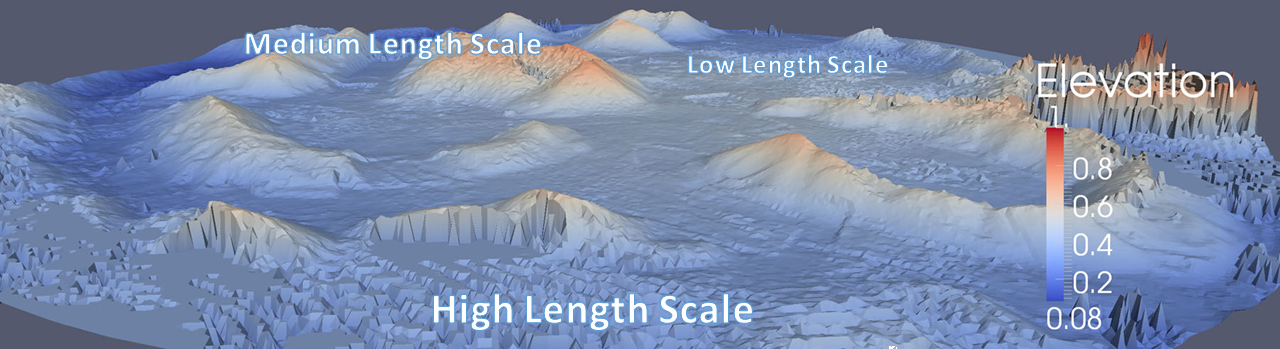
\includegraphics[width=\textwidth]{Figures/gaussianprocesslengthscale.png}
					\caption{Non-stationary Gaussian process for seafloor terrain modeling Adapted from \cite{ROB:ROB21403}}
					\label{Figure:GaussianProcessLengthScale}
				\end{figure}
				
				The non-stationary kernel function employed in this thesis is the Paciorek non-stationary covariance kernel function \eqref{Equation:NonStationaryKernel} \citep{AdaptiveNonStationaryKernel}.
				
				\begin{equation}
					k(\bvec{x}_{i}, \bvec{x}_{j}) = \sigma_{f}^{2} |\Sigma_{i}|^{\frac{1}{4}} |\Sigma_{j}|^{\frac{1}{4}} \Bigg|\frac{\Sigma_{i} + \Sigma_{j}}{2}\Bigg|^{-\frac{1}{2}} \exp\Bigg[ -\frac{1}{2} (\bvec{x}_{i} - \bvec{x}_{j}) \Bigg(\frac{\Sigma_{i} + \Sigma_{j}}{2}\Bigg)^{-1} (\bvec{x}_{i} - \bvec{x}_{j}) \Bigg]
				\label{Equation:NonStationaryKernel}
				\end{equation}			
				
				The matrices $\Sigma_{i}$ and $\Sigma_{j}$ are the local length scale matrices at $\bvec{x}_{i}$ and $\bvec{x}_{j}$ respectively, and are interpreted the same way as the stationary case. The only difference is that these length scale matrices only operate locally, and are functions of the input feature vector $\bvec{x}$. In each kernel location, two length scale matrices are queried. Hence, in a kernel matrix of size $n \times m$, maximally $n + m$ unique queries are made if no feature locations overlap.
				
				It is worthwhile to observe that the effective length scale matrix in the exponent is the average of the two length scale matrices, with its effect reduced with increasing distance between the two points of consideration as with all kernels.
				
				Note that the normalisation matrix determinants are chosen such that the kernel function is reduced into the squared exponential stationary kernel when $\Sigma_{i} = \Sigma_{j} = \Sigma$, as derived in \eqref{Equation:NonStationaryKernelToStationaryKernel}. 
		
				That is, the Paciorek non-stationary kernel reduces to the squared exponential kernel under the stationary limit. In this way, the Paciorek kernel generalises the squared exponential kernel.
						
				\begin{equation}
					\left.
						\begin{aligned}
							k(\bvec{x}_{i}, \bvec{x}_{j}) &= \sigma_{f}^{2} |\Sigma|^{\frac{1}{4}} |\Sigma|^{\frac{1}{4}} \Bigg|\frac{\Sigma + \Sigma}{2}\Bigg|^{-\frac{1}{2}} \exp\Bigg[ -\frac{1}{2} (\bvec{x}_{i} - \bvec{x}_{j}) \Bigg(\frac{\Sigma + \Sigma}{2}\Bigg)^{-1} (\bvec{x}_{i} - \bvec{x}_{j}) \Bigg] \\
							&= \sigma_{f}^{2} |\Sigma|^{\frac{1}{2}} |\Sigma|^{-\frac{1}{2}} \exp\Bigg[ -\frac{1}{2} (\bvec{x}_{i} - \bvec{x}_{j}) (\Sigma)^{-1} (\bvec{x}_{i} - \bvec{x}_{j}) \Bigg] \\
							&= \sigma_{f}^{2} \exp\Bigg[ -\frac{1}{2} (\bvec{x}_{i} - \bvec{x}_{j}) \Sigma^{-1} (\bvec{x}_{i} - \bvec{x}_{j}) \Bigg]
						\end{aligned}
					\qquad \right.
				\label{Equation:NonStationaryKernelToStationaryKernel}
				\end{equation}		
			
		\subsection{Regression}
		\label{Background:GaussianProcesses:Regression}
		
			Gaussian process regression is a regression technique that employs Gaussian processes as its inference model. Because Gaussian processes already operate on function spaces with continuous inputs and outputs, no extra pre-processing or transformations are needed. The bulk of the technique thus lies in learning the kernel function of the Gaussian process. Gaussian process regression is also called \textit{kriging} or Kolmogorov Wiener prediction when used for interpolating geospatial data in a geostatistics setting. This section attempts to summarise the important concepts regarding GP regression and how they work.
			
			Once a kernel function is chosen, such as the squared exponential or \matern kernels, learning the kernel function becomes equivalent to learning the hyperparameters of the kernel. In this way, the Gaussian process model is defined completely by its hyperparameters $\vec{\uptheta}$. % , which are often only handful in quantity. % This illustrates that while its temporal complexity $\mathcal{O}(n^{3})$ is quite high, its spatial complexity and memory requirements are quite moderate at $\frac{m(m + 1)}{2} + 1 + n(m  + 1)$ real numbers, where $n(m  + 1)$ real numbers comes from the training data itself. % Minimally, after assuming a particular kernel functional form, the bulk of the model information is held by the data set itself. Especially in big data applications, unlike generalised linear models and neural networks whose information vector \footnote{The information vector is the vector of all parameters that defines the model.} is proportional to the number of basis functions employed, a Gaussian process model can have its information stored by a few hyperparameters.
			
			Before presenting the inference process for Gaussian process regression however, it is important to understand the way Gaussian processes are used in general for Bayesian inference, which applies to both regression and classification.
			
			\subsubsection{General Gaussian Process Inference Process}
			
				The formulation for Gaussian processes from definitions \ref{Definition:GaussianProcess} and \ref{Definition:GaussianRandomField} provides an framework for inferring the behaviour of an unknown function $f(\bvec{x})$. In general, however, the output target does not have to be the functional outputs $f := f(\bvec{x})$. Instead, the output targets are some quantity $y$ which can be directly observed and recorded. The function $f$ serves as an intermediate step to infer $y$ from $\bvec{x}$, and in general cannot be directly observed. Therefore, the function $f$ is also called the \textit{latent function}.
				
				% Define block styles
				\tikzstyle{line} = [draw, -latex']
				\tikzstyle{cloud1} = [draw, ellipse, fill = green!30!blue!30, node distance = 3cm, minimum height = 3em,  minimum width = 5em]
				\tikzstyle{cloud2} = [draw, ellipse, fill = green!60!blue!50, node distance = 3cm, minimum height = 3em,  minimum width = 5em]
				
				\begin{figure}[!ht]
				\centering\makebox[\textwidth]{
					\begin{tikzpicture}[node distance = 4cm, auto, comment/.style ={rectangle, inner sep = 2pt, text width = 4cm, }]
					
					\node [cloud1] (trainingfeatures) {$X$};
					\node [cloud2, right of = trainingfeatures] (traininglatents) {$\bvec{f}$};
					\node [cloud1, right of = traininglatents] (trainingtargets) {$\bvec{y}$};
					\node [cloud2, below of = traininglatents] (querylatents) {$\bvec{f}^{\star}$};
					\node [cloud1, left of = querylatents] (queryfeatures) {$X^{\star}$};
					\node [cloud2, right of = querylatents] (querytargets) {$\bvec{y}^{\star}$};
					
					\draw [line] (trainingfeatures) -- (traininglatents);
					\draw [line] (traininglatents) -- (trainingtargets);
					\draw [line] (traininglatents) -- (querylatents);
					\draw [line] (queryfeatures) -- (querylatents);
					\draw [line] (querylatents) -- (querytargets);	
					\end{tikzpicture}
					}		
				\caption{Gaussian Process Graphical Model}
				\label{Figure:GaussianProcessGraphicalModel}
				\end{figure}
				
				This inference process can be visualised with the graphical model presented in Figure \ref{Figure:GaussianProcessGraphicalModel}. Observed and known quantities are coloured in blue. Quantities to be inferred are coloured in green. Note that in a Bayesian model, the unknown quantities (in green) are inferenced by their probabilistic distributions, and not just their estimated values.
				
				Latent functions are usually interpreted as the underlying phenomenon which stochastically generates the target outputs $y$.  The model assumes that a particular phenomenon $f$ is responsible for generating the output target $y$, and that the phenomenon $f$ can be explained reasonably by a particular set of features $\bvec{x}$. A collection of output targets $\bvec{y}$ and corresponding features $X$ are observed. The collected dataset $(X, \bvec{y})$ is termed the \textit{training data}. A \textit{learning process} then occurs where the model learns the underlying phenomenon $\bvec{f}$ at the training points. If the learning process is done through an optimisation procedure in search for an optimal model in some quantifiable sense, the learning process is also termed a \textit{training process}. An \textit{inference process} then occurs where the model is to infer the latent process $\bvec{f}^{\star}$ at the query features $X^{\star}$, which would further allow inference on the corresponding target outputs $\bvec{y}^{\star}$. The inference process in general also includes the act of inferring related quantities regarding the distribution of $\bvec{y}^{\star}$. Typical examples include inferring the uncertainty involved in the inference stage through a variance or entropy measure. If the only quantity to be inferenced is the expected target outputs $\mathbb{E}[\bvec{y}^{\star} | \bvec{y}]$, then the inference process is also termed a \textit{prediction process}. In this way, the GP modeling process is composed of two stages - the learning or training stage and the inference or prediction stage.
				
				A typical example in the regression case is a situation where the observable outputs $y$ are related to the underlying phenomenon $f(x)$ through a simple white noise process \eqref{Equation:RegressionNoiseModelScalar}.
				
				\begin{equation}
					y_{i} = f(\bvec{x}_{i}) + \epsilon_{i} \qquad \epsilon_{i} \sim \mathcal{N}(0, \sigma^{2}) \qquad \forall i \in I_{n}
				\label{Equation:RegressionNoiseModelScalar}
				\end{equation}
				
				In general, however, the relationship between the output target $y$ and the latent functional $f$ is captured through a likelihood response $p(y | f)$, which captures the likelihood of generating a particular output target $y$ \textit{if} the latent functional is $f$. In fact, the choice of the likelihood function is not immediately straightforward and is of vital importance in the classification scenario. 
				
				In the regression model above \eqref{Equation:RegressionNoiseModelScalar}, a degenerate case arises when the noise level $\sigma$ is zero such that $y = f$ everywhere. In this case, $p(y | f) = p(f | f) = 1$ such that the Gaussian process model performs inference on the target output directly through obtaining $p (y) = p(f)$. When this is not the case, however, the quantity to be inferred in the end is the output targets $y$. As such, the distribution of interest is $p(y)$. This can be obtained by marginalising away the latent functionals $f$ over the likelihood $p(y | f)$ \eqref{Equation:Marginalisation}.
				
				\begin{equation}
					p(y) = \int_{\mathscr{F}} p(y | f) p(f) df
				\label{Equation:Marginalisation}
				\end{equation}
				
				where $\mathscr{F}$ is the space of all latent functionals. Note that the form \eqref{Equation:Marginalisation} above is written in functional form to illustrate the relevant concepts. The marginalisation process above plays a vital process in the learning stage for Gaussian process inference discussed shortly.
		
			\subsubsection{Inference}
			
				The above general inference process can now be formulated specifically for the regression case.
				
				With a given kernel function $k$ as the covariance function, by definition \ref{Definition:GaussianRandomField} we have that the training latents $\bvec{f}$ and the query latents $\bvec{f^{\star}}$ are distributed as a multivariate Gaussian \eqref{Equation:InferenceJointDistribution}.
				
				\begin{equation}
					\begin{bmatrix}
						\bvec{f^{ }} \\ \bvec{f^{\star}}
					\end{bmatrix}
					\sim \mathcal{N}\Bigg(\bvec{0}, \begin{bmatrix}
														K(X, X) & K(X, X^{\star}) \\
														K(X^{\star}, X) & K(X^{\star}, X^{\star}) \\
													\end{bmatrix}  \Bigg)
				\label{Equation:InferenceJointDistribution}
				\end{equation}
				
				% where the matrix $K(X, X')$ is defined to have elements $K_{ij} = k(\bvec{x}_{i}, \bvec{x}'_{j})$ with $X$ and $X'$ defined as the canonical data design matrix form \eqref{Background:GaussianProcess:Equation:DataMatrix}, both of each can take either the matrix of training points $X$ of size $n$ or query points $X^{\star}$ of size $n^{\star}$.
				
				To shorten notation, it is customary to define $K := K(X, X)$, $K^{\star} := K(X, X^{\star})$, $K^{\star \star} := K(X^{\star}, X^{\star})$, where the symmetry of the covariance matrix readily yields ${K^{\star}}^{T} := K(X^{\star}, X)$. In this thesis, $K$ will be referred to as the \textit{data kernel} or \textit{training kernel}, $K^{\star}$ as the \textit{inference kernel}, and $K^{\star \star}$ as the \textit{query kernel}.
				
				\begin{equation}
					X = \{\bvec{x}_{i}\}_{i \in I_{n}}^{T} := \begin{bmatrix}
						\bvec{x}_{1}^{T} \\ \bvec{x}_{2}^{T} \\ \dots \\ \bvec{x}_{n}^{T}
					\end{bmatrix} \qquad X' = \{\bvec{x'}_{i}\}_{i \in I_{n}}^{T} := \begin{bmatrix}
										\bvec{x'}_{1}^{T} \\ \bvec{x'}_{2}^{T} \\ \dots \\ \bvec{x'}_{n}^{T}
									\end{bmatrix}
				\label{Equation:TrainingQueryDataMatrices}
				\end{equation}	
					
				The joint distribution readily contains information for the conditional distribution of the query points given the training points $p(\bvec{f^{\star}} | \bvec{f})$ knowing the training points and query locations. This leads to the posterior distribution \eqref{Equation:InfereceConditionalDistribution}. Note that in some literature, the feature locations $X$ and $X^{\star}$ are also included in the conditioned set, so that the conditional distribution is written as $\bvec{f^{\star}} | \bvec{f}, X, X^{\star}$. However, throughout this thesis, since the feature locations $X$ and $X^{\star}$ are always known, they are inherently conditioned upon and will not be shown explicitly in notation for consise presentation. 
				
				\begin{equation}
					\bvec{f^{\star}} | \bvec{f} \sim \mathcal{N}({K^{\star}}^{T} K^{-1} \bvec{f}, K^{\star \star} - {K^{\star}}^{T} K^{-1} K^{\star})
				\label{Equation:InfereceConditionalDistribution}
				\end{equation}						
				
				A comparison with the prior $\bvec{f^{\star}} \sim \mathcal{N}(\bvec{0}, K^{\star \star})$ shows the mean effect ${K^{\star}}^{T} K^{-1} \bvec{f}$ and covariance effect $- {K^{\star}}^{T} K^{-1} K^{\star}$ which introduces observed information into the model. Interestingly, as ${K^{\star}}^{T} K^{-1} K^{\star}$ is positive definite, this intuitively means that the observation has reduced uncertainty in the model.
				
				The above posterior formulation encompasses the heart of the GP regression model. The rest of the discussion will focus on detailed aspects of its implementation and variants.
				
				% \subsubsection{Noisy Observations}
				
				Under noisy observations, a hyperparameter $\sigma$ is introduced for the standard deviation of the noise, which is also assumed to be \textit{iid} and Gaussian distributed with standard deviation $\sigma$ and zero mean. The only alteration is the observations are notated as $\bvec{y}$ instead of $\bvec{f}$, where 
				
				\begin{equation}
					\bvec{y}(X) = \bvec{f}(X) + \bvec{\upepsilon} \qquad \bvec{\upepsilon} \sim \mathcal{N}(\bvec{0}, \sigma^{2} I_{n \times n})
				\label{Equation:RegressionNoiseModel}
				\end{equation}
							
				and most importantly the data kernel is to be replaced with $K \mapsto K + \sigma^{2} I$. Note that however the query points remain as the latent function $\bvec{f^{\star}}$. If one were to predict future observations $\bvec{y^{\star}}$, then it suffices to generate $\bvec{f^{\star}}$ from the posterior and add randomly generated noise with standard deviation $\sigma$.
				
			\subsubsection{Hyperparameter Learning}
			\label{Background:GaussianProcess:Regression:HyperparameterLearning}
			
				One of the most important yet tricky aspects of GP modeling is the training stage. Since the model is determined entirely by the hyperparameters, the hyperparameters must be optimised in accordance to some fitness metric. The fitness metric employed to be maximised is the marginal likelihood, otherwise termed as evidence, of the observed data. This is usually non-trivial to compute and, in most cases, analytical forms do not exist. Fortunately, due to the Gaussian structure of the GP model, there exists an analytical form for the marginal likelihood. In practice, however, it is computationally faster to compute the log marginal likelihood \eqref{Background:GaussianProcess:Equation:LogMarginalLikelihood}.
				
				\begin{equation}
					\log(p(\bvec{f})) = - \frac{1}{2} \bvec{f}^{T} K^{-1} \bvec{f} - \frac{1}{2} \log|K| - \frac{n}{2} \log(2 \pi)
				\label{Background:GaussianProcess:Equation:LogMarginalLikelihood}
				\end{equation}
				
				Again, with noisy observations, corresponding substitutions with the data kernel matrix $K \mapsto K + \sigma^{2} I$ and observations $\bvec{f} \mapsto \bvec{y}$ is to be made.
				
				The last term is a constant, so it can be ignored during the optimisation stage and included back in once optimisation completes.
				
				In practice, hyperparameter learning can be sped up by employing the fact that $\frac{1}{2} \log|K| = \sum_{i} L_{ii} = \mathrm{trace}(L)$ where $L$ is the Cholesky decomposition of $K$ (or $K + \sigma^{2} I$ in the noisy case). In fact, the Cholesky decomposition $L$ leads to better numerical stability when inverting the matrix $K$ since $K = LL^{T}$ so that $K \backslash \bvec{y} = L^{T} \backslash (L \backslash \bvec{y})$.
				
		\subsection{Classification}
		\label{Background:GaussianProcesses:Classification}
		
			The GP classification method is of vital importance to the benthic habitat modeling process. It is used to distinguish and predict the environment type with a measure of entropy in order to quantify the information reward one can gain by exploring the area.
			
			Unlike the regression case, because the output labels are no longer continuous, it cannot be represented by a continuous probability density function such as a Gaussian. As such, a continuous latent function is introduced in the GP classification process. Intuitively, this latent function quantifies and measures the distinct qualities of the label. As a binary classification example, if the classifier is to distinguish between ``apples'' and ``oranges'', the latent function would then represent the ``appleness'' of each observation, with high ``appleness'' corresponding to observations likely to be ``apples'' and low ``appleness'' corresponding to observations likely to be ``oranges''. Note that only one latent function is needed in the binary case. The latent function is then monotonically ``squashed'' into the unit range [0, 1] so that it can be interpreted as a probability.
			
			Although the latent function is now continuous such that it is possible to model it with a GP regression model, the posterior probability is in general non-Gaussian distributed, since the ``squashing'' is usually non-linear such that the likelihood is non-Gaussian. In this way, approximations are necessary. Four of the most popular approximations to GP classification, in increasing accuracy and computational complexity, are Probabilistic Least Squares, Laplace Approximation, Expectation Propagation, and Variational Inference \citep{GaussianProcessForMachineLearning}. In this thesis, Laplace approximation is chosen as a reasonable balance between accuracy and implementation difficulty, although a short investigation of probabilistic least squares will also be provided.
			
			\subsubsection{Response Functions}
			\label{Background:GaussianProcesses:Classification:ResponseFunction}
			
				Before discussions begin regarding the various types of GP classifiers, it is important to understand the role of \textit{response functions} in Bayesian classifiers.
				
				The response function is sometimes also called a sigmoid function, and are used as the likelihood model for Bayesian classifiers. These functions must satisfy the requirement that is it monotonically non-decreasing with a domain of all real numbers $\mathbb{R}$ and a range of unit interval [0, 1]. That is, $\lambda(z): \mathbb{R} \mapsto [0, 1]$. As referenced above, these functions serve to "squeeze" the latent functions into a range where probabilistic interpretation is possible.
				
				The most widely used response functions are the logistic function \eqref{Equation:LogisticResponse} and probit \footnote{The probit function is also simply the standard normal cumulative distribution. The term \textit{probit} is used to make explicit its interpretation as a response likelihood function.} response \eqref{Equation:ProbitResponse} (figure \ref{Figure:LikelihoodResponses}).
				
				\begin{equation}
					\lambda(z) = \frac{1}{1 + \exp(-z)}
				\label{Equation:LogisticResponse}
				\end{equation}
				
				\begin{equation}
					\lambda(z) = \Phi(z) := \int\limits_{-\infty}^{z} \phi(x) dx =  \int\limits_{-\infty}^{z} \frac{1}{\sqrt{2 \pi}} \exp\Big(- \frac{1}{2} x^{2}\Big) dx
				\label{Equation:ProbitResponse}
				\end{equation}
			
				\begin{figure}[!htbp]
					\centering
						\includegraphics[width=0.75\textwidth]{Figures/responses.eps}
					\caption{Common likelihood responses}
					\label{Figure:LikelihoodResponses}
				\end{figure}
				
			\subsubsection{Binary Classification}
			\label{Background:GaussianProcesses:Classification:BinaryClassification}
			
				The Laplace approximation for GP binary classification works by learning a latent function through an iterative scheme involving successive GP regressions, and "squeezing" that latent function into an appropriate probabilistic range for likelihood interpretation. The Laplace approximation approaches the approximation problem by determining the mean and variance of the true distribution and approximating the said distribution with a Gaussian distribution of the same mean and variance. Assuming Gaussian distributions, the prior and the evidence (marginal likelihood) have analytical forms. Under such assumptions it is therefore possible to marginalise out the likelihood predictions to obtain a posterior estimate. Finally, this learning stage can be trained by optimising the marginal likelihood \footnote{{\color{BurntOrange} At this stage of the thesis progress, it is uncertain whether or not a deeper and more rigorous theoretical grounding should be provided for GP classification. Perhaps it would benefit by only providing an intuitive outline of the procedure, rather than a rigorous derivation, so that the reader is not distracted from the main contributions of this thesis later on.}}.
				
			\subsubsection{Laplace Approximation}
			\label{Background:GaussianProcesses:Classification:LaplaceApproximation}
			
			\subsubsection{Probabilistic Least Squares}
			\label{Background:GaussianProcesses:Classification:ProbabilisticLeastSquares}
			
			\subsubsection{Multiclass Classification: One v.s. All}
			\label{Background:GaussianProcesses:Classification:OVA}
			
				While a consistent framework for the GP Multi-class classification using Laplace approximation exist, a simpler and perhaps a more computationally efficient approach is to employ the One v.s. All (OVA) and All v.s. All (AVA) philosophy. The following discussion assumes that there are $c > 2$ classes of labels for which classification is to occur. 
				
				The OVA approach performs classification by introducing $c$ \textit{independent} classification problems, each trying to classify a label against all others. Each of these problems are thus a binary classification problem for which solution methods are known. Once the predictive probabilities from all learned GP classifiers are obtained, a consistent framework is used for fusing the separate prediction probabilities into a coherent prediction probability. This is necessary as the binary classifiers are independently learned and performs prediction independently, and may not necessarily provide coherent results. In fact, simply stacking the prediction probabilities together yields a "probability" distribution that does not sum up to 1.
				
				The AVA approach operates similarly. It insteads introduces $\frac{c (c - 1)}{2}$ \textit{independent} classification problems, each classifying between a pair of labels. The same exact philosophy follows in that a final consistent framework is needed for fusing the prediction probabilities into one coherent prediction probability. It is often more difficult for probability fusion in the AVA setting as compared to the OVA setting.
			
			\subsubsection{Multiclass Classification: All v.s. All}
			\label{Background:GaussianProcesses:Classification:AVA}
			
			\subsubsection{Fusion of Prediction Probability}
			\label{Background:GaussianProcesses:Classification:ProbabilityFusion}
			
				{\color{BurntOrange} This section should be in the GP implementation chapter of this thesis (e.g. Chapter 3). It would further the discussion above regarding the probability fusion problem by introducing the exclusion method and mode keeping method that has been developed and tested. It is anticipated that other methods will be developed by then, so that this section would undergo significant editing.}
				
				
				
	%				The main decision and analysis to be made in both the OVA and AVA setting is the framework for which the probabilities are to be fused. 
	%							
	%				The exclusion method centers around the idea that the probabilities are to be made consistent by eliminating, or excluding, the events that are impossible.
	%				
	%				Consider a single query point for which class prediction is to occur. Let $\pi_{i}$ be the prediction probability obtained through the binary classification of class $i$ against all other classes. Initially, the probability vector $\bvec{\pi} := [\pi_{1}, \pi_{2}, \dots, \pi_{c}]^{T}$ is not a unit vector, so that $\bvec{\pi}$ does not define a proper probability distribution \dots 
		
			\subsubsection{Entropy}
			\label{Background:GaussianProcesses:Classification:Entropy}
			
				After a predictive probability distribution is obtained for each query environment location, the uncertainty of such predictions can be quantified through the entropy of of that distribution.
				
				The output of a GP classifier is a discrete probability distribution with finite size - equal to the number of classes. For a general discrete probability distribution $p(x)$, the entropy is quantified as below \eqref{Equation:DiscreteEntropy} \cite{ShannonEntropy}.
				
				\begin{equation}
					H(p) = - \sum_{i} p(x_{i}) \log(p(x_{i}))
				\label{Equation:DiscreteEntropy}
				\end{equation}
				
				Although it is unlikely that the entropy of bathymetric feature modeling is required, the regression posterior is a continuous probability density $p(x)$ for which a similar form for distribution entropy exists \eqref{Equation:ContinuousEntropy}.
				
				\begin{equation}
					H(p) = - \int_{\Omega_{x}} p(x) \log(p(x)) dx
				\label{Equation:ContinuousEntropy}
				\end{equation}
								
				With these entropy measures, predictive uncertainties can be quantified, which allows active information seeking plans to be possible.
				
			\subsubsection{Sampling from a Gaussian Process for Classifiers}
			\label{Background:GaussianProcesses:Classification:Sampling}
			
	\section{Active Sampling}
	\label{Background:ActiveSampling}
	
		\subsection{Static Active Sampling}
		\label{Background:ActiveSampling:Static}
		
		\subsection{Dynamic Active Sampling}
		\label{Background:ActiveSampling:Dynamic}
		
	\section{Informative Path Planning}
	\label{Background:InformativePathPlanning}
	
		Path planning under dynamic uncertainty has been a challenging task for all information searching missions. This class of path planning problems have the special property that there is no goal location, and no stationary node, edge, or field cost to be cumulatively minimised. The objective is to reduce the overall uncertainty or entropy of a particular region given indefinite time. The complication is introduced with the non-linear dynamics of the uncertainty or entropy field of the region each time a planned path is executed, which also makes the solution extremely frequency dependent.
		
		Prior work and attempts at the active path planning problem include Marchant and Ramos (2014), where Bayesian Optimisation (BO) techniques combined with Gaussian process models are employed in an environmental monitoring setting \citep{BayesianOptimisation}. In this layered Bayesian Optimisation approach, two Gaussian processes are used - one to model the phenomenon and the other to model the quality of selected paths. Through Bayesian optimisation, sampling over continuous paths are optimised which maximises the reward over the final mission trajectory. The path planning process is done using Markov Decision Processes (MDP) with a Reinforcement Learning approach. Rapidly Exploring Random Graphs (RRGs) is combined with BO to search for informative paths. In this way, a continuous path can be planned through BO \citep{BayesianOptimisation}.
		
		This was was further extended by Marchant et. al. (2014) where Sequential Bayesian Optimisation (SBO) is used as online POMDPs for path planning \citep{SequentialBayesianOptimisation}.
		
		Other prior work includes Brooks et. al. (2006) where the POMDP approach is investigated for continuous state space planning \citep{ParametricPOMDP}. This method was compared to previous work with value-based and gradient-based solution methods which seek to transcribe the continuous problem into a discrete problem \footnote{{\color{BurntOrange} The author has practiced with transcribing the continuous problem into a discrete problem in a shortest path setting in}}. One of the most important limitations discussed in this work is that analytical and accurate solutions exist almost only for linear systems with quadratic cost (Linear Quadratic Systems). Otherwise, the other option with non-value based methods require heuristics that can be difficult to justify for its appropriateness to the problem. Nevertheless, through parametrising the problem, parametric POMDPs can provide an accurate solution to the path planning problem under certain assumption such as linear quadratic dynamics \citep{ParametricPOMDP}.
		
		In conclusion, POMDP methods are currently one of the most reliable and accurate method for continuous path planning in an information gathering setting. While the technique enforces limitations on the problem dynamics, with sufficient modeling it is deemed possible to perform path planning to an acceptable level. This thesis will thus investigate POMDP methods for active path planning in the ocean exploration setting.
		
		\subsection{Myopic and Non-myopic Planning}
		\label{Background:InformativePathPlanning:MyopicNonmyopicPlanning}
		
		\subsection{Advantages of Gaussian Process Models}
		\label{Background:InformativePathPlanning:GaussianProcessAdvantage}
		
		

\lhead{Building Gaussian Process Classifiers}
\chapter{Building Gaussian Process Classifiers}
\label{BuildingGaussianProcessClassifiers}
	

	Gaussian processes (GP) are stochastic processes which generalises the multi-variate Gaussian distribution. In a statistical learning and machine learning context, they are categorised as a type of \textit{supervised learning} method, which describes the problem of learning relationships between input and output variables from empirical data. The empirical data is also often referred to as the training set.
	
	Supervised learning methods are often further categorised into regression and classification problems, depending on the nature of the output variable. The problem is a regression problem if the output is continuous, and a classification problem if the output is discrete. In the ocean environment modeling setting, bathymetric modeling is a regression problem (when feature extraction is infeasible), and environment type prediction is a classification problem.
	
	In both regression and classification settings, the input variables are often also referred to as \textit{features}, which motivated the term "bathymetric features" in the previous sections - especially to distinguish it from the spatial inputs. In statistical literature, continuous regression outputs are sometimes called \textit{response} variables, although it is more often simply referred as the \textit{output} or \textit{target} in the machine learning community. Discrete classification outputs are referred to as \textit{labels}. In this context, \textit{environment type} and \textit{environment labels} are synonymous. 
	
	In the sections which references the use of Gaussian process models, $\bvec{x}$ will denote the input variable or features of the problem while $y$ will denote the output or target variable. Note that in general there are multiple features such that the input is a feature vector $\bvec{x}$. Without loss of generality, however, the output variable can always be treated as a scalar quantity $y$. Under cases of multiple output variables, the problem can be split into multiple single output variable problems. It is true that prediction performance can actually be improved by considering the output vector together, which leads to multi-task regression, as will be briefly discussed. Nevertheless, the main bulk of the content revolve around single output Gaussian processes.
	
	The work presented here will be primarily based on Rasmussen and William's work in \textit{Gaussian Process for Machine Learning} from 2006 \cite{GaussianProcessForMachineLearning}. 

	\section{Bayesian Modeling with Gaussian Processes}
	\label{Background:GaussianProcesses:BayesianModeling}
	
		The Gaussian process formulation follows the Bayesian modeling philosophy. An important distinction Bayesian modeling makes from the classical approach is the idea of estimating a distribution instead of a point value. While this is often more computationally expensive, it provides a very robust and accurate framework for prediction and analysis. More importantly, it provides capabilities that classical approaches do not possess - the ability to quantify prediction uncertainties. 
		
		The basic Bayesian modeling process begins with a prior distribution $p(H)$, the probability distribution of prediction model $H$ being representative, and updates this to a posterior distribution $p(H | D)$, the updated probability distribution of prediction model $H$ being representative after observing a particular data set $D$ \footnote{This discussion employs the common notational convention that the event of observing $D$ is also named $D$, and the event of model $H$ being the most representative is also named $H$.}. 
		
		This procedure is illustrated in \cref{Background:OceanEnvironmentModeling:Figure:bayesianmodeling}, where the posterior is updated by two observations. This example further serves to illustrate the concept of distributions over functions, which behaves as an infinite-dimensional generalisation of a multi-variate probability distribution. Instead of drawing random finite vectors from distributions, a random function is drawn from a \textit{process}, a term used to refer to infinite \footnote{When the input variable is temporal, a process can be more realistically interpreted as having indefinite dimensional distributions.} dimensional multi-variate distributions. It is helpful to conceptualise functions as an infinite string of points, such that drawing from an infinite dimensional distribution is equivalent to drawing from processes that operate on function space.
		
		\begin{figure}[!htbp]
			\centering
				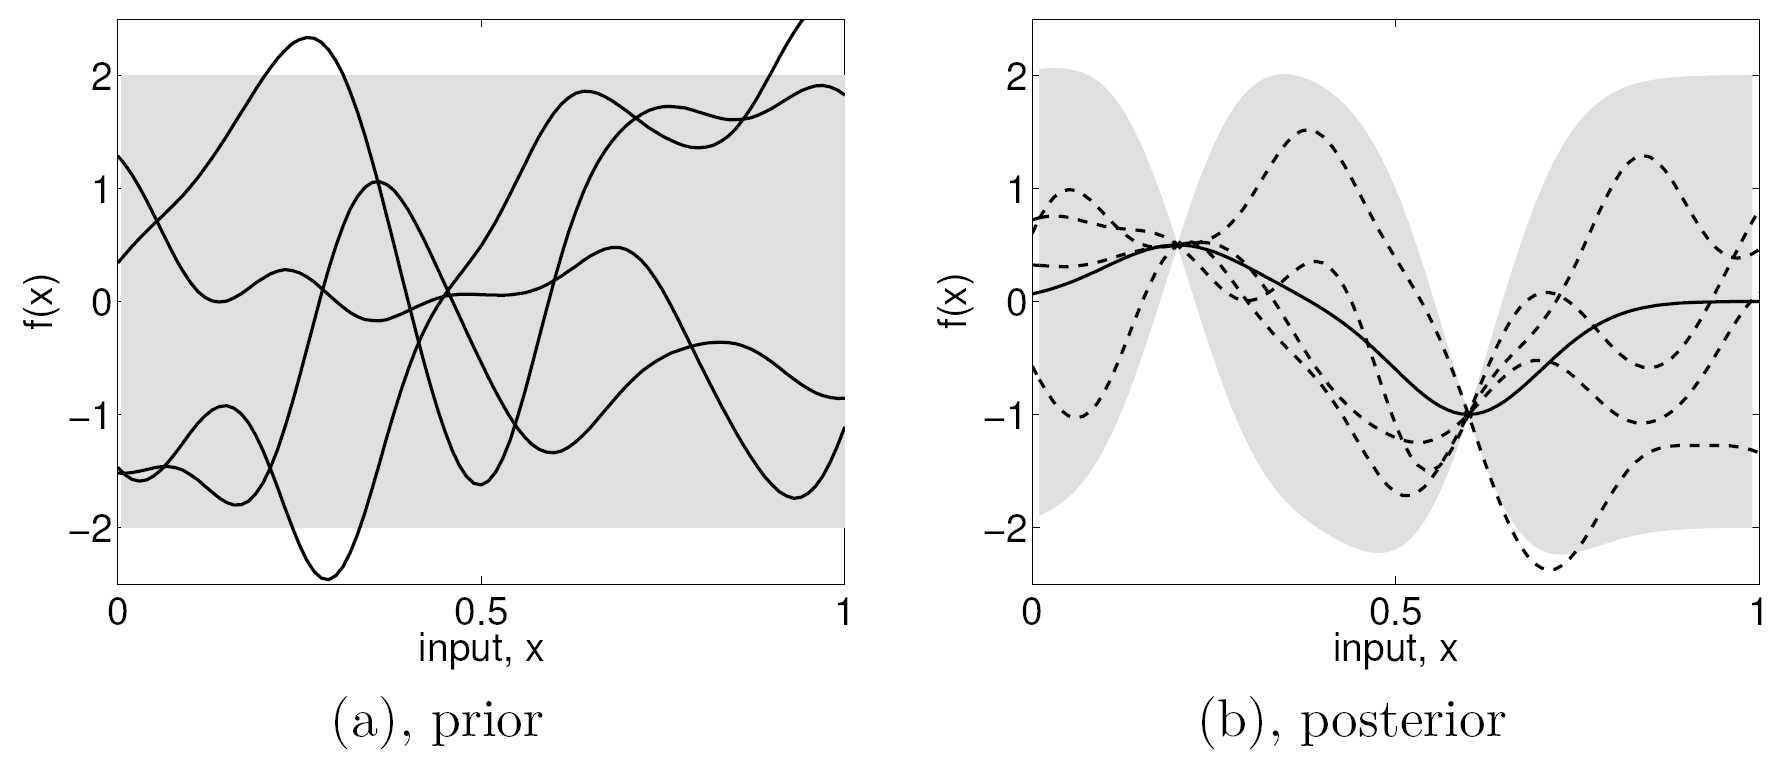
\includegraphics[width=0.9\textwidth]{Figures/bayesianmodeling.png}
			\caption{Illustration of Gaussian Process Bayesian Modeling: The mean prediction is shown as the solid line. Four samples are drawn in each case, represented by the dashed line. The shared region represents the 2-$\sigma$ bounds of the prediction at each input feature value $x$. Two points are observed which updated the distribution from the prior to the posterior.\\
			Figure (a) shows the situation for the prior distribution.\\
			Figure (b) shows the situation for the posterior distribution. \\
			Source: Rasmussen and Williams (2006) \cite{GaussianProcessForMachineLearning}}
			\label{Background:OceanEnvironmentModeling:Figure:bayesianmodeling}
		\end{figure}
		
		From this illustration, there are a few qualities one can notice. Firstly, the prior distribution is simply the zero function. The prior is meant to represent the system's current belief before the next observations are to be made. In this case, the prior situation involves no observations at all. Ideally, this means that the prior distribution should contain no predictive information. However, it is of philosophical note that all informative \footnote{It is certainly possible to perform inference without any assumptions. It will simply be uninformative in prediction or result.} inferences must start off with some assumptions regarding the structure of this problem. In the illustration above, the function is assumed to be distributed as a process with zero mean. This assumption has excluded processes without means, such as the Cauchy process, as well as assumed a rather arbitrary mean function. However, this assumption is often valid as one can always pre-process the output data set through subtracting off their empirical mean so that the output is distributed about zero. The representation of the variance functions as confidence bounds centered at the mean function also hints that multi-model processes are excluded. In fact, the illustration shows a Gaussian process, which is indeed uni-modal - just as its finite dimensional form.
		
		Speaking of the variance, a second observation is that the standard deviation and hence variance of the output function decreases at the observations, and gradually increases away from the observations. This leads to two remarks. Firstly, the variance or uncertainty of the output function at a location reduces when observations are made at that location. Secondly, neighboring points are related - the closer they are, the more related they are. This is seen through the observed points dragging nearby points towards it while reducing the uncertainty of nearby points. This resembles the concept of covariance. Evidently, points closer to each other have higher covariance then those further away, and the covariance beween the same points simply become its variance.
		
		The two observations above demonstrate that, just as a Gaussian distribution is defined through a mean vector and a covariance matrix, a Gaussian process is defined through a mean function $m(x)$ and a covariance function $k(x, x')$. In Gaussian process literature, the covariance function is also called a \textit{kernel} function.
		
		Formally, a function $f(x)$ is distributed as a Gaussian process $f(x) \sim \mathcal{GP}(m(x), k(x, x'))$ if for any finite collection of points $\bvec{x} := [x_{1}, x_{2}, \dots, x_{n}]^{T}$, the corresponding output vector $f(\bvec{x}) := [f(x_{1}), f(x_{2}), \dots, f(x_{n})]^{T}$ is jointly distributed as a multi-variate Gaussian such that $f(\bvec{x}) \sim \mathcal{N}(\bvec{m}(\bvec{x}), K(\bvec{x}, \bvec{x}'))$. Certainly, this is true for finite dimensional multi-variate Gaussian distributions, in that any subset of a said distributed random vector will also be multi-variate Gaussian distributed of lower dimensionality. The next few sections will discuss the kernel matrix $K$ more rigorously.
		
		Finally, as mentioned before, the mean function can be generally assumed to be the zero function, as at each stage of inference both the model and data can be subtracted by their theoretical or empirical means. This elucidates that Gaussian processes are completely defined by their kernel function $k$. 
		
		\FloatBarrier
		
	\section{Kernel Functions}
	\label{Background:GaussianProcesses:KernelFunctions}
	
		\subsection{Stationary Kernels}
		
			As kernel functions completely define the prediction characteristics of a Gaussian process, this section aims to provide the mathematical background regarding kernels that are necessary for understanding Gaussian processes. The following discussion will only cover the minimal background necessary for further sections, as treatments of kernel functions can easily become very detailed and rigorous once analysis begins in topics such as differentiability effects or eigenfunction decomposition. Further treatment of this material is available through Rasmussen and Williams (2006) \cite{GaussianProcessForMachineLearning}. 
			
			Intuitively, the kernel function determines the \textit{similarity} between data points. This is a notion that all supervised learning algorithms intend to do, although rather implicitly in most cases. The $\mathcal{GP}$ formulation makes this explicit through the covariance between any two points in the feature space.
			
			Kernel functions can be categorised into stationary kernels and non-stationary kernels. In this thesis, non-stationary kernels will become of vital importance in bathymetric and environment modeling. 
			
			Stationary kernels are ones whose covariance properties do not depend explicitly on the locations $\bvec{x}$ and $\bvec{x}'$ of consideration, but only on the difference $\bvec{x} - \bvec{x}'$ between them. Thus, the covariance properties are \textit{stationary}, or invariant, under translations in the feature space.
			
			Common stationary kernels are the squared exponential kernel \footnote{Squared exponential kernels are also sometimes called Gaussian kernels. However, in conversations it tends to create confusion between the probability density function $\phi(x)$ for Gaussian distributions and the covariance function $k(x, x')$ itself, so this term is avoided in this thesis.} and the \matern kernels. The squared exponential (SE) kernel between any two points $\bvec{x}, \bvec{x}' \in \mathbb{R}^{m}$ in the feature space with $m$ features has the following form \eqref{Background:GaussianProcess:Equation:SquaredExponentialKernel}.
			
			\begin{equation}
				\left.
					\begin{aligned}
						k_{\mathrm{SE}}(\bvec{x}, \bvec{x}') &= \sigma_{f}^{2} \exp\Big(-\frac{1}{2}(\bvec{x} - \bvec{x}')^{T} \Sigma^{-1} (\bvec{x} - \bvec{x}')\Big) = \sigma_{f} \exp\Big(-\frac{1}{2} a^{2} \Big) \\
						\Sigma &= 	\begin{bmatrix}
										l_{1}^{2} & l_{12} & \dots & l_{1m} \\
										l_{21}^{2} & l_{2}^{2} & \dots & l_{2m} \\
										\vdots & \vdots  & \ddots & \vdots \\
										l_{m1}^{2} & l_{m2} & \dots & l_{m}^{2} \\
								  	\end{bmatrix}
					\end{aligned}
				\qquad \right.
			\label{Background:GaussianProcess:Equation:SquaredExponentialKernel}
			\end{equation}
			
			Here, $\sigma_{f}$ is called the sensitivity, and determines the overall reference strength scale of the covariance function. The matrix $\Sigma$ is the length scale matrix, and determines the reference length scale and principle axis directions within the feature space. Like most quadratic forms, $\Sigma$ is required to be symmetric and positive semi-definite. In particular, when $\Sigma$ is diagonal, the kernel is termed \textit{axis aligned}. When $\Sigma$ is proportional to an identity such that $\Sigma = l^{2} I_{m \times m}$, the kernel is termed \textit{isotropic}.
			
			The sensitivity parameter $\sigma_{f}$ and length scale parameters $l_{ij}$, $i, j \in {1, 2, \dots, m}$ with $l_{i} := l_{ii}$ completely withhold the information of a squared exponential kernel. Unlike parametric models, however, while these parameters define the kernel directly, they define the $\mathcal{GP}$ model indirectly. Because of the multiple levels of relation from these parameters to the model, these parameters are termed \textit{hyperparameters} of the $\mathcal{GP}$.
			
			In practice, it is often possible to pre-process the data or transform the feature space so that an axis aligned kernel can be applied. The assumption imposed is that the principle axis directions are aligned with the feature space axis. In this case, the $\mathcal{GP}$ model is defined by $m + 1$ hyperparameters, where $m$ is the number of features. Even without the axis-aligned assumption, the number of hyperparameters is $\frac{m(m + 1)}{2} + 1$.
			
			The above formulation suggests to define $a^{2} := (\bvec{x} - \bvec{x}')^{T} \Sigma^{-1} (\bvec{x} - \bvec{x}')$. This can be interpreted as the squared distance between $\bvec{x}$ and $\bvec{x}'$ under the warp defined by $\Sigma$. In particular, when the feature space is isotropic such that $\Sigma = l^{2} I_{m \times m}$, then $a = \frac{r}{l}$ where $r := +\sqrt{r^{2}}$, $l := +\sqrt{l^{2}}$, and $r^{2} = (\bvec{x} - \bvec{x}')^{T} (\bvec{x} - \bvec{x}')$. In fact, most stationary kernels are functions solely of $a^{2}$, or with the definition $a := +\sqrt{a^{2}}$, they are simply scalar functions with scalar inputs $a = a (\bvec{x}, \bvec{x'})$. This form also makes evident that the covariances between two points decreases monotonically as the distance between them increases - a property most kernel functions exhibit.
			
			Continuing with this formulation, the \matern class of kernel functions are given by \eqref{Background:GaussianProcess:Equation:MaternKernel}.
			
			\begin{equation}
				\left.
					\begin{aligned}
						k_{\mathrm{\maternmath}}(\bvec{x}, \bvec{x}') =& \; \sigma_{f}^{2} \frac{2^{1 - \nu}}{\Gamma(\nu)} \Big( \sqrt{2 \nu} a \Big)^{\nu} K_{\nu}\Big( \sqrt{2 \nu} a \Big) \\
						a^{2} :=& \; (\bvec{x} - \bvec{x}')^{T} \Sigma^{-1} (\bvec{x} - \bvec{x}')
					\end{aligned}
				\qquad \right.
			\label{Background:GaussianProcess:Equation:MaternKernel}
			\end{equation}
						
			$\Gamma$ and $K_{\nu}$ are the Gamma function and modified Bessel function respectively \cite{GaussianProcessForMachineLearning}. $\nu$ is a positive hyperparameter that determines the differentiability property of the \matern class kernel. The $\mathcal{GP}$ model with \matern class kernel is $d$-times mean square differentiable if and only if $\nu > k$. In the limit of $\nu \rightarrow \infty$ for infinite differentiability, the \matern kernel becomes the squared exponential kernel \eqref{Background:GaussianProcess:Equation:SquaredExponentialKernel}. While the general \matern class kernel seem complicated due to the Gamma function and modified Bessel function, its form become simple for $\nu = p + \frac{1}{2}$ where $p$ is a non-negative integer. That is, \matern kernels with $\nu = \frac{1}{2}, \frac{3}{2}, \frac{5}{2}, \frac{7}{2}, \dots$ have simple analytic forms without reference to the modified Bessel function. In fact, for $\nu > \frac{5}{2}$, the degree for which the \matern kernel changes becomes quite unnoticeable for most practical purposes such that it may as well be replaced by the squared exponential kernel with $\nu \rightarrow \infty$. Similarly, while there is a more noticeable effect of changing $\nu$ within the range $\nu \in (0, \frac{5}{2})$, in practice is it is often not worth the expense of implementing the complicated form for a almost unnoticeable improvement in modeling accuracy. Hence, it is replaced with the \matern kernel $\nu = \frac{1}{2}, \frac{3}{2}, \frac{5}{2}$, whichever is the closest. In this way, in practice only the \matern kernels with $\nu = \frac{1}{2}, \frac{3}{2}, \frac{5}{2}$ are employed, and they are respectively termed the \matern 1/2 kernel, \matern 3/2 kernel, and \matern 5/2 kernel - in the order of increasing differentiability. These kernels have forms as listed below \eqref{Background:GaussianProcess:Equation:PracticalMaternKernels}.
			
			\begin{equation}
				\left.
					\begin{aligned}
						k_{\mathrm{\maternmath}, \; \nu = \frac{1}{2}}(\bvec{x}, \bvec{x}') =& \; \sigma_{f}^{2} \exp ( -a ) \\
						k_{\mathrm{\maternmath}, \; \nu = \frac{3}{2}}(\bvec{x}, \bvec{x}') =& \; \sigma_{f}^{2} (1 + \sqrt{3} a) \exp ( -\sqrt{3} a ) \\
						k_{\mathrm{\maternmath}, \; \nu = \frac{5}{2}}(\bvec{x}, \bvec{x}') =& \; \sigma_{f}^{2} \Big(1 + \sqrt{5} a + \frac{5}{3} a^{2}\Big) \exp ( -\sqrt{5} a )  \\
						a^{2} :=& \; (\bvec{x} - \bvec{x}')^{T} \Sigma^{-1} (\bvec{x} - \bvec{x}')
					\end{aligned}
				\qquad \right.
			\label{Background:GaussianProcess:Equation:PracticalMaternKernels}
			\end{equation}			
			
			Together, the squared exponential kernel and the \matern class kernels provide a flexible set of kernel functions that can model a multitude of phenomena from various fields such as geology, ecology, finance, logistics, control theory, and machine learning. Specifically, kernel functions make spatial relations explicit which assists in the interpretation in spatial modeling cases, including bathymetric modeling and ocean environment modeling.
		
		\subsection{Non-Stationary Kernels}
			
			Non-stationary kernels introduce flexibility for modeling phenomenons where the inherent length scales varies across feature locations. The problem with stationary kernels is that the GP will always learn length scales that are as small as it needs to for modeling the fastest varying phenomenon in the model. While the marginal likelihood inherently balances modeling accuracy and overfitting, when it comes to the choice between modeling a peak in data variation with a risk of overfitting the rest of the data or ignoring that peak, the optimiser will always prefer the former as marginal likelihood gain from successful modeling is higher than loss from overfitting. Because learning stage is done through optimising the marginal likelihood, this forces the length scale to be smaller than it needs at slower varying places.

			Figure \ref{Background:GaussianProcess:Figure:gaussianprocesslengthscale} illustrates the non-stationary Gaussian process for a terrain modeling application. Note that this does not imply that it is only relevant for GP regression problems - the latent functions used in GP classification is itself a GP regression problem for which length scale interpretation is almost identical to that shown in \cref{Background:GaussianProcess:Figure:gaussianprocesslengthscale}.
			
			\begin{figure}[!htbp]
				\centering
					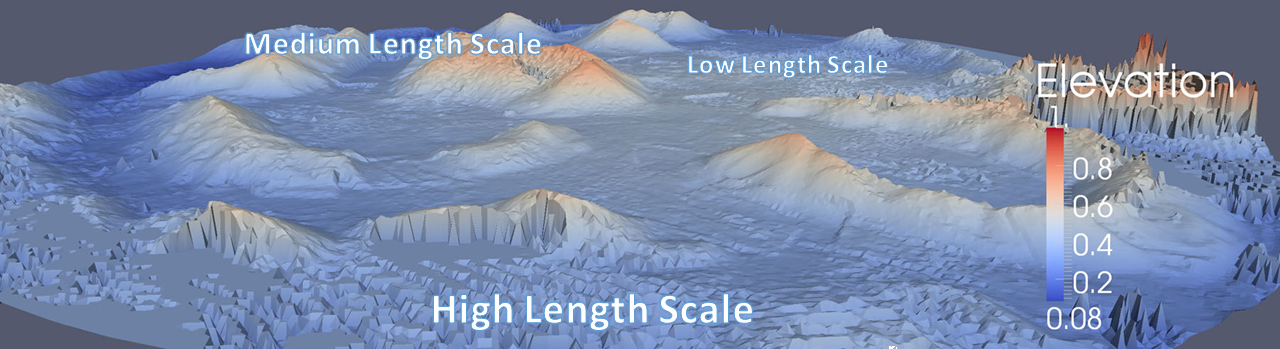
\includegraphics[width=\textwidth]{Figures/gaussianprocesslengthscale.png}
				\caption{Illustration of non-stationary Gaussian process for terrain modeling \cite{GaussianProcessTerrainFigure} \\
				Flat parts have high length scales (slow varying) while \\ rough parts have low length scales (fast varying)}
				\label{Background:GaussianProcess:Figure:gaussianprocesslengthscale}
			\end{figure}
			
			The non-stationary kernel function employed is the Paciorek Non-Stationary Covariance Function \eqref{Background:GaussianProcess:Equation:NonStationaryKernel} \cite{AdaptiveNonStationaryKernel}.
			
			\begin{equation}
				k(\bvec{x}_{i}, \bvec{x}_{j}) = \sigma_{f}^{2} |\Sigma_{i}|^{\frac{1}{4}} |\Sigma_{j}|^{\frac{1}{4}} \Bigg|\frac{\Sigma_{i} + \Sigma_{j}}{2}\Bigg|^{-\frac{1}{2}} \exp\Bigg[ -\frac{1}{2} (\bvec{x}_{i} - \bvec{x}_{j}) \Bigg(\frac{\Sigma_{i} + \Sigma_{j}}{2}\Bigg)^{-1} (\bvec{x}_{i} - \bvec{x}_{j}) \Bigg]
			\label{Background:GaussianProcess:Equation:NonStationaryKernel}
			\end{equation}			
			
			The matrices $\Sigma_{i}$ and $\Sigma_{j}$ are the local length scale matrices at $\bvec{x}_{i}$ and $\bvec{x}_{j}$ respectively, and are interpreted the same way as the stationary case. The only difference is that these length scale matrices only operate locally, and are functions of the input feature vector $\bvec{x}$. In each kernel location, two length scale matrices are queried. Hence, in a kernel matrix of size $n \times m$, around $n + m$ unique queries are made if no feature locations overlap.
			
			It is worthwhile to observe that the effective length scale matrix in the exponent is the average of the two length scale matrices, with its effect reduced with increasing distance between the two points of consideration as with all kernels.
			
			Note that the normalisation matrix determinants are chosen such that the kernel function is reduced into a stationary one when $\Sigma_{i} = \Sigma_{j} = \Sigma$ \eqref{Background:GaussianProcess:Equation:NonStationaryKernelToStationary}. 
			
			\begin{equation}
				\left.
					\begin{aligned}
						k(\bvec{x}_{i}, \bvec{x}_{j}) &= \sigma_{f}^{2} |\Sigma|^{\frac{1}{4}} |\Sigma|^{\frac{1}{4}} \Bigg|\frac{\Sigma + \Sigma}{2}\Bigg|^{-\frac{1}{2}} \exp\Bigg[ -\frac{1}{2} (\bvec{x}_{i} - \bvec{x}_{j}) \Bigg(\frac{\Sigma + \Sigma}{2}\Bigg)^{-1} (\bvec{x}_{i} - \bvec{x}_{j}) \Bigg] \\
						k(\bvec{x}_{i}, \bvec{x}_{j}) &= \sigma_{f}^{2} |\Sigma|^{\frac{1}{2}} |\Sigma|^{-\frac{1}{2}} \exp\Bigg[ -\frac{1}{2} (\bvec{x}_{i} - \bvec{x}_{j}) (\Sigma)^{-1} (\bvec{x}_{i} - \bvec{x}_{j}) \Bigg] \\
						k(\bvec{x}_{i}, \bvec{x}_{j}) &= \sigma_{f}^{2} \exp\Bigg[ -\frac{1}{2} (\bvec{x}_{i} - \bvec{x}_{j}) \Sigma^{-1} (\bvec{x}_{i} - \bvec{x}_{j}) \Bigg]
					\end{aligned}
				\qquad \right.
			\label{Background:GaussianProcess:Equation:NonStationaryKernelToStationary}
			\end{equation}		
			
			That is, the Paciorek non-stationary kernel reduces to the squared exponential kernel under the stationary limit. In this way, the Paciorek kernel generalises the squared exponential kernel.
			
			
			\FloatBarrier
		
	\section{Regression}
	\label{Background:GaussianProcesses:Regression}
	
		Gaussian process regression is a regression technique that employs Gaussian processes as its inference model. Because Gaussian processes already operate on function spaces with continuous inputs and outputs, no extra pre-processing or transformations are needed. The bulk of the technique thus lies in learning the kernel function of the Gaussian process. Gaussian process regression is also called \textit{kriging} or Kolmogorov Wiener prediction when used for interpolating geospatial data in a geostatistics setting. This section attempts to summarise the important concepts regarding $\mathcal{GP}$ regression and how they work. More rigorous discussions are available from Rasmussen and Williams (2006) \cite{GaussianProcessForMachineLearning}. 
		
		Once a kernel function is chosen, such as the squared exponential or \matern kernels, learning the kernel function becomes equivalent to learning the hyperparameters of the kernel. In this way, the Gaussian process model is actually defined completely by its hyperparameters, which are often only handful in quantity. This illustrates that while its temporal complexity $\mathcal{O}(n^{3})$ is quite high, its spatial complexity and memory requirements are quite moderate at $\frac{m(m + 1)}{2} + 1 + n(m  + 1)$ real numbers, where $n(m  + 1)$ real numbers comes from the training data itself. % Minimally, after assuming a particular kernel functional form, the bulk of the model information is held by the data set itself. Especially in big data applications, unlike generalised linear models and neural networks whose information vector \footnote{The information vector is the vector of all parameters that defines the model.} is proportional to the number of basis functions employed, a Gaussian process model can have its information stored by a few hyperparameters.
		
		With a given kernel function $k$ as the covariance function, by definition we have that the training observations $\bvec{f}$ and the query observations $\bvec{f^{\star}}$ is distributed as a multivariate Gaussian \eqref{Background:GaussianProcess:Equation:Distribution}.
		
		\begin{equation}
			\begin{bmatrix}
				\bvec{f^{ }} \\ \bvec{f^{\star}}
			\end{bmatrix}
			\sim \mathcal{N}\Bigg(\bvec{0}, \begin{bmatrix}
												K(X, X) & K(X, X^{\star}) \\
												K(X^{\star}, X) & K(X^{\star}, X^{\star}) \\
											\end{bmatrix}  \Bigg)
		\label{Background:GaussianProcess:Equation:Distribution}
		\end{equation}
		
		where the matrix $K(X, X')$ is defined to have elements $K_{ij} = k(\bvec{x}_{i}, \bvec{x}'_{j})$ with $X$ and $X'$ defined as the canonical data design matrix form \eqref{Background:GaussianProcess:Equation:DataMatrix}, both of each can take either the matrix of training points $X$ of size $n$ or query points $X^{\star}$ of size $n^{\star}$. To shorten notation, it is customary to define $K := K(X, X)$, $K^{\star} := K(X, X^{\star})$, $K^{\star \star} := K(X^{\star}, X^{\star})$, where the symmetry of the covariance matrix readily yields ${K^{\star}}^{T} := K(X^{\star}, X)$. Specifically, $K$ will be referred to as the data kernel.
		
		\begin{equation}
			X = \begin{bmatrix}
				\bvec{x}_{1}^{T} \\ \bvec{x}_{2}^{T} \\ \dots \\ \bvec{x}_{n}^{T}
			\end{bmatrix} \qquad X' = \begin{bmatrix}
								\bvec{x'}_{1}^{T} \\ \bvec{x'}_{2}^{T} \\ \dots \\ \bvec{x'}_{n}^{T}
							\end{bmatrix}
		\label{Background:GaussianProcess:Equation:DataMatrix}
		\end{equation}	
			
		The joint distribution readily contains information for the conditional distribution of the query points given the training points $p(\bvec{f^{\star}} | \bvec{f})$ knowing the training points and query locations \footnote{Throughout this thesis, since the feature locations $X$ and $X^{\star}$ are always known, they are inherently conditioned upon and will not be shown explicitly in notation.}. This leads to the posterior distribution \eqref{Background:GaussianProcess:Equation:ConditionalDistribution}.
		
		\begin{equation}
			\bvec{f^{\star}} | \bvec{f} \sim \mathcal{N}({K^{\star}}^{T} K^{-1} \bvec{f}, K^{\star \star} - {K^{\star}}^{T} K^{-1} K^{\star})
		\label{Background:GaussianProcess:Equation:ConditionalDistribution}
		\end{equation}						
		
		A comparison with the prior $\bvec{f^{\star}} \sim \mathcal{N}(\bvec{0}, K^{\star \star})$ shows the mean effect ${K^{\star}}^{T} K^{-1} \bvec{f}$ and covariance effect $- {K^{\star}}^{T} K^{-1} K^{\star}$ which introduces observed information into the model. Interestingly, as ${K^{\star}}^{T} K^{-1} K^{\star}$ is positive definite, this intuitively means that the observation has reduced uncertainty in the model.
		
		The above posterior formulation encompasses the heart of the GP regression model. The rest of the discussion will focus on detailed aspects of its implementation and variants.
		
		% \subsection{Noisy Observations}
		
		Under noisy observations, a hyperparameter $\sigma$ is introduced for the standard deviation of the noise, which is also assumed to be \textit{iid} and Gaussian distributed with standard deviation $\sigma$ and zero mean. The only alteration is the observations are notated as $\bvec{y}$ instead of $\bvec{f}$, and most importantly the data kernel is to be replaced with $K \mapsto K + \sigma^{2} I$. Note that however the query points remain as the latent function $\bvec{f^{\star}}$. If one were to predict future observations $\bvec{y^{\star}}$, then it suffices to generate $\bvec{f^{\star}}$ from the posterior and add randomly generated noise with standard deviation $\sigma$.
			
		\subsection{Hyperparameter Learning}
		
			One of the most important yet tricky aspects of GP modeling is the training stage. Since the model is determined entirely by the hyperparameters, the hyperparameters must be optimised in accordance to some fitness metric. The fitness metric employed to be maximised is the marginal likelihood, otherwise termed as evidence, of the observed data. This is usually non-trivial to calculate and, in most cases, analytical forms do not exist. Fortunately, due to the Gaussian assumption of he GP model, there exists an analytical form for the marginal likelihood. In practice, however, it is computationally faster to compute the log marginal likelihood \eqref{Background:GaussianProcess:Equation:LogMarginalLikelihood}.
			
			\begin{equation}
				\log(p(\bvec{f})) = - \frac{1}{2} \bvec{f}^{T} K^{-1} \bvec{f} - \frac{1}{2} \log|K| - \frac{n}{2} \log(2 \pi)
			\label{Background:GaussianProcess:Equation:LogMarginalLikelihood}
			\end{equation}
			
			Again, with noisy observations, corresponding substitutions with the data kernel matrix $K \mapsto K + \sigma^{2} I$ and observations $\bvec{f} \mapsto \bvec{y}$ is to be made.
			
			The last term is a constant, so it can be ignored during the optimisation stage and included back in once optimisation completes.
			
			In practice, hyperparameter learning can be sped up by employing the fact that $\frac{1}{2} \log|K| = \sum_{i} L_{ii} = \mathrm{trace}(L)$ where $L$ is the Cholesky decomposition of $K$ (or $K + \sigma^{2} I$ in the noisy case). In fact, the Cholesky decomposition $L$ leads to better numerical stability when inverting the matrix $K$ since $K = LL^{T}$ so that $K \backslash \bvec{y} = L^{T} \backslash (L \backslash \bvec{y})$.
		
		\subsection{Sampling from a Gaussian Process}
		
%			\subsection{Multi-task Regression}
%			
%				Multi-task regression operates on the same principles as the single-task regression. With multiple outputs, each output is assigned to a single-task regression problem as discussed above. However, a covariance matrix between each output is kept track of such that each output can perform inference on other outputs as well.
%				
%				The advantage of this approach is that different outputs recorded at different feature positions can assist each other to fill in each other's data gap. In this way, the over all entropy can be reduced.
%				
%				In an environment modeling setting, the main problem that occurs even after a good model has been learned is that entropy always increases at places where there is less data, as opposed to places that are inherently interesting and high in entropy even after observations. Multi-tasking improves the situation by lowering the entropy at those places with scarce data but inherently uninteresting.
			
	\section{Classification}
	\label{Background:GaussianProcesses:Classification}
	
		The GP classification method is of vital importance to the environment modeling process. It is used to distinguish and predict the environment type with a measure of entropy in order to quantify the information reward one can gain by exploring the area.
		
		Unlike the regression case, because the output labels are no longer continuous, it cannot be represented by a continuous probability density function such as a Gaussian. As such, a continuous latent function is introduced in the GP classification process. Intuitively, this latent function quantifies and measures the distinct qualities of the label. As a binary classification example, if the classifier is to distinguish between "Apples" and "Oranges", the latent function would then represent the "Appleness" of each observation, with high "Appleness" corresponding to observations likely to be "Apples" and low "Appleness" corresponding to observations likely to be "Oranges". Note that only one latent function is needed in the binary case. The latent function is then "squashed" into the unit range [0, 1] so that it can be interpreted as a probability.
		
		Although the latent function is now continuous such that it is possible to model it with a GP regression model, the posterior probability is in general non-Gaussian distributed. In this way, approximations are necessary.
		
		There exists four approximate methods for GP classification. In increasing orders of accuracy and decreasing order of implementation difficulty, they are Probabilistic One Nearest Neighbor (P1NN), Laplace Approximation (LP), Expectation Propagation (EP), and Gaussian Process Least Squares Classifier (GPLSC) \cite{GaussianProcessForMachineLearning}. In this section, Laplace approximation is chosen as a reasonable balance between accuracy and implementation difficulty.
		
		\subsection{Response Functions}
		
			Before discussions begin regarding the various types of GP classifiers, it is important to understand the role of \textit{response functions} in Bayesian classifiers.
			
			The response function is sometimes also called a sigmoid function. These functions must satisfy the requirement that is it monotonically non-decreasing with a domain of all real numbers $\mathbb{R}$ and a range of unit interval [0, 1]. That is, $\lambda(z): \mathbb{R} \mapsto [0, 1]$. As referenced above, these functions serve to "squeeze" the latent functions into a range where probabilistic interpretation is possible.
			
			The most widely used response function is with no doubt the logistic function \eqref{Background:GaussianProcess:Equation:Logistic}. Response functions that are also commonly used in a GP classifier setting include the normal cumulative distribution function \eqref{Background:GaussianProcess:Equation:normalcdf}.
			
			\begin{equation}
				\lambda(z) = \frac{1}{1 + \exp(-z)}
			\label{Background:GaussianProcess:Equation:Logistic}
			\end{equation}
			
			\begin{equation}
				\lambda(z) = \Phi(z) := \int\limits_{-\infty}^{z} \phi(x) dx =  \int\limits_{-\infty}^{z} \frac{1}{\sqrt{2 \pi}} \exp\Big(- \frac{1}{2} x^{2}\Big) dx
			\label{Background:GaussianProcess:Equation:normalcdf}
			\end{equation}
			
		\subsection{Binary Classification}
		
			The Laplace approximation for GP binary classification works by learning a latent function through an iterative scheme involving successive GP regressions, and "squeezing" that latent function into an appropriate probabilistic range for likelihood interpretation. The Laplace approximation approaches the approximation problem by determining the mean and variance of the true distribution and approximating the said distribution with a Gaussian distribution of the same mean and variance. Assuming Gaussian distributions, the prior and the evidence (marginal likelihood) have analytical forms. Under such assumptions it is therefore possible to marginalise out the likelihood predictions to obtain a posterior estimate. Finally, this learning stage can be trained by optimising the marginal likelihood \footnote{{\color{BurntOrange} At this stage of the thesis progress, it is uncertain whether or not a deeper and more rigorous theoretical grounding should be provided for GP classification. Perhaps it would benefit by only providing an intuitive outline of the procedure, rather than a rigorous derivation, so that the reader is not distracted from the main contributions of this thesis later on.}}.
			
		\subsection{Laplace Approximation}
			
		\subsection{Probabilistic Least Squares}
		
		\subsection{Multiclass Classification: One v.s. All}
		
			While a consistent framework for the GP Multi-class classification using Laplace approximation exist, a simpler and perhaps a more computationally efficient approach is to employ the One v.s. All (OVA) and All v.s. All (AVA) philosophy. The following discussion assumes that there are $c > 2$ classes of labels for which classification is to occur. 
			
			The OVA approach performs classification by introducing $c$ \textit{independent} classification problems, each trying to classify a label against all others. Each of these problems are thus a binary classification problem for which solution methods are known. Once the predictive probabilities from all learned GP classifiers are obtained, a consistent framework is used for fusing the separate prediction probabilities into a coherent prediction probability. This is necessary as the binary classifiers are independently learned and performs prediction independently, and may not necessarily provide coherent results. In fact, simply stacking the prediction probabilities together yields a "probability" distribution that does not sum up to 1.
			
			The AVA approach operates similarly. It insteads introduces $\frac{c (c - 1)}{2}$ \textit{independent} classification problems, each classifying between a pair of labels. The same exact philosophy follows in that a final consistent framework is needed for fusing the prediction probabilities into one coherent prediction probability. It is often more difficult for probability fusion in the AVA setting as compared to the OVA setting.
		
		\subsection{Multiclass Classification: All v.s. All}
			
		\subsection{Fusion of Prediction Probability}

			{\color{BurntOrange} This section should be in the GP implementation chapter of this thesis (e.g. Chapter 3). It would further the discussion above regarding the probability fusion problem by introducing the exclusion method and mode keeping method that has been developed and tested. It is anticipated that other methods will be developed by then, so that this section would undergo significant editing.}
			
			
			
%				The main decision and analysis to be made in both the OVA and AVA setting is the framework for which the probabilities are to be fused. 
%							
%				The exclusion method centers around the idea that the probabilities are to be made consistent by eliminating, or excluding, the events that are impossible.
%				
%				Consider a single query point for which class prediction is to occur. Let $\pi_{i}$ be the prediction probability obtained through the binary classification of class $i$ against all other classes. Initially, the probability vector $\bvec{\pi} := [\pi_{1}, \pi_{2}, \dots, \pi_{c}]^{T}$ is not a unit vector, so that $\bvec{\pi}$ does not define a proper probability distribution \dots 
	
		\subsection{Entropy}
		
			After a predictive probability distribution is obtained for each query environment location, the uncertainty of such predictions can be quantified through the entropy of of that distribution.
			
			The output of a GP classifier is a discrete probability distribution with finite size - equal to the number of classes. For a general discrete probability distribution $p(x)$, the entropy is quantified as below \eqref{Background:GaussianProcess:Equation:DiscreteEntropy}.
			
			\begin{equation}
				H(p(x)) = - \sum_{i} p(x_{i}) \log(p(x_{i}))
			\label{Background:GaussianProcess:Equation:DiscreteEntropy}
			\end{equation}
			
			Although it is unlikely that the entropy of bathymetric feature modeling is required, the regression posterior is a continuous probability density $p(x)$ for which a similar form for distribution entropy exists \eqref{Background:GaussianProcess:Equation:ContinuousEntropy}.
			
			\begin{equation}
				H(p(x)) = - \int_{\Omega_{x}} p(x) \log(p(x)) dx
			\label{Background:GaussianProcess:Equation:ContinuousEntropy}
			\end{equation}
							
			With these entropy measures, predictive uncertainties can be quantified, which allows active information seeking plans to be possible.
			
		\subsection{Sampling from a Gaussian Process for Classifiers}
		

		




\lhead{Modeling the Ocean Environment}
\chapter{Modeling the Ocean Environment}
\label{ModelingOceanEnvironment}

%	\section{Gaussian Process Classification with Laplace Approximation}
%	
%%		\subsection{Theory}
%%		
%%		\subsection{Implementation}
%%		
%%		\subsection{Results}
%		
%	\section{Gaussian Process Classification with Probabilistic Least Squares}
%
%%		\subsection{Theory}
%%		
%%		\subsection{Implementation}
%%			
%%		\subsection{Results}
%		
%	\section{Non Stationary GP Classification}
%	
%%		\subsection{Theory}
%%		
%%		\subsection{Implementation}
%%			
%%		\subsection{Results}
%		
%	\section{Drawing from Gaussian Process Classifiers}
%				
%%		\subsection{Theory}
%%		
%%		\subsection{Implementation}
%%			
%%		\subsection{Results}
			
	\section{Modeling Features}
	\label{ModelingOceanEnvironment:ModelingFeatures}
	
		This thesis project can be broken down into two main parts - ocean environment modeling and path planning. Ocean environment modeling itself includes bathymetric feature extraction and modeling, and environment label modeling. This section will focus on the environment modeling aspect.
			
		In order for autonomous underwater vehicles to plan a path that can maximise the amount of information gained regarding a particular ocean region, it would need a method to predict the types of environments it may encounter, with a measure of its prediction uncertainty.
		
		While the path planner is to plan in the spatial space, in general the prediction model operates upon some feature space with more direct and explicit relationships with the output we would like to predict.
		
		It is thus important to make a distinction between the feature space $F$ for which label modeling is to occur and the spatial space $S$ for which bathymetric modeling and planning is to occur. The spatial space usually consists of Cartesian coordinates $(x, y)$ in the eastings-northings frame or the longitude-latitude frame. The path is to be planned in this spatial space. The frame is usually converted into a local body frame during the execution of control signals for path tracking. However, this does not affect the formulation presented here. The feature space includes bathymetric features for which the labels will be modeled upon. Depending on the features employed for the modeling process, there are usually approximate analytical forms for extracting such features from raw depth observations.

		The following features in \cref{Background:OceanEnvironmentModeling:Table:Features} were chosen by the author for bathymetric modeling. 

		\begin{table}[h]
			\begin{center}
				\begin{tabular}{ |c|c|c| }
					\hline
					Feature Name & Feature Symbol & Feature Units \\
					\hline
					Depth & $h$ & m \\
					Slope (Small Scale) & $m_{s}$ & m/m \\
					Slope (Large Scale) & $m_{l}$& m/m \\
					Rugosity (Small Scale) & $r_{s}$ & $\mathrm{m^{2}/m^{2}}$ \\
					Rugosity (Large Scale) & $r_{l}$ & $\mathrm{m^{2}/m^{2}}$  \\
					\hline
				\end{tabular}
			\end{center}
	  	\caption{Bathymetric Features}
	  	\label{Background:OceanEnvironmentModeling:Table:Features}			
	  	\end{table}	
		
		The raw bathymetric data contains depth information at various spatial locations. Such data are often collected rather uniformly in approximate grid formations such that it is possible to calculate the ocean floor slope through finite differencing. The slope is divided into small scale and large scale variations, as marine environments - especially underwater habitats - often depend not only on the immediate slope but also slope variations on the larger scale. The same idea applies to rugosity, the measure of local height variations. The feature extraction process is detailed in \cref{Background:OceanEnvironmentModeling:FeatureExtraction}. 
		  
		Spatial coordinates are chosen to be excluded from the bathymetric feature set. For environment prediction purposes, it is expected that ecological habitats and geological sites exhibit no explicit relationship with the location of the site, and that its properties arise solely due to the local environment characteristics (features) of that site.
		
		\FloatBarrier			
		
		Figure \ref{Background:OceanEnvironmentModeling:Figure:modelingprocess} show a high level overview of the ocean environment modeling process. As bathymetric data is available in more quantities and distributed more uniformly, it is often sufficient to employ the feature extraction process outlined in \cref{Background:OceanEnvironmentModeling:FeatureExtraction} to obtain the bathymetric features for modeling. However, if the bathymetric data is sufficiently sparse or is not distributed uniformly for grid based methods, then the feature extraction process itself becomes a prediction problem.

		\begin{figure}[!htbp]
			\centering
				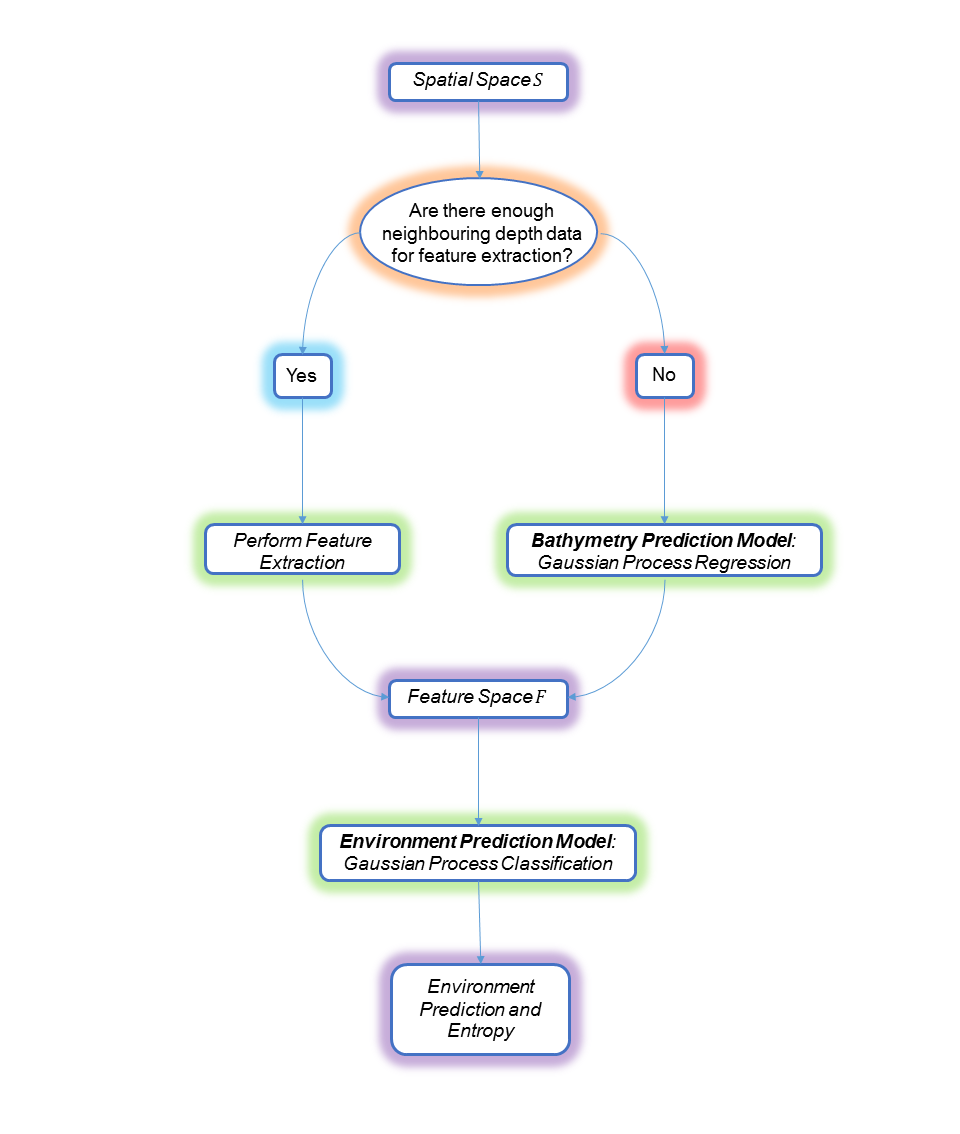
\includegraphics[width=\textwidth]{Figures/modelingprocess.png}
			\caption{Environment Modeling}
			\label{Background:OceanEnvironmentModeling:Figure:modelingprocess}
		\end{figure}
				
		In that case, a Gaussian process regression model is proposed for predicting the features at a given spatial location. While this is much more computationally expensive than performing feature extraction, it is also quite rare that this is necessary under abundant bathymetric data.
		
		Finally, once the feature vectors are obtained at training locations, the environment type is to be predicted. The environment type is summarised through labels that indicate the type of marine environment that was observed or predicted. Common AUV mission examples include "reef", "sand", and "rocks". These labels are often summarised through processing visual and stereo imagery obtained through past AUV missions. With a discrete set of possible labels, the environment prediction problem is to be modeled as a Gaussian process classification problem. From here on, the environment prediction problem is understood to refer to the two stage process of feature extraction or modeling and environment label prediction, with the latter being the main bottleneck for this process.
		
		\FloatBarrier
		
		\subsection{Environment Modeling - Data Matching}
		\label{Background:OceanEnvironmentModeling:DataMatching}
		
			A subtlety that arises from the above formulation is that during the training stage, the bathymetric data and the label data are not necessarily observed at the same places. Figure \ref{Background:OceanEnvironmentModeling:Figure:illustrationBathymetricAgainstLabels} illustrates the spatial distribution of the two datasets in a typical setting.
		
			\begin{figure}[!htbp]
				\centering
					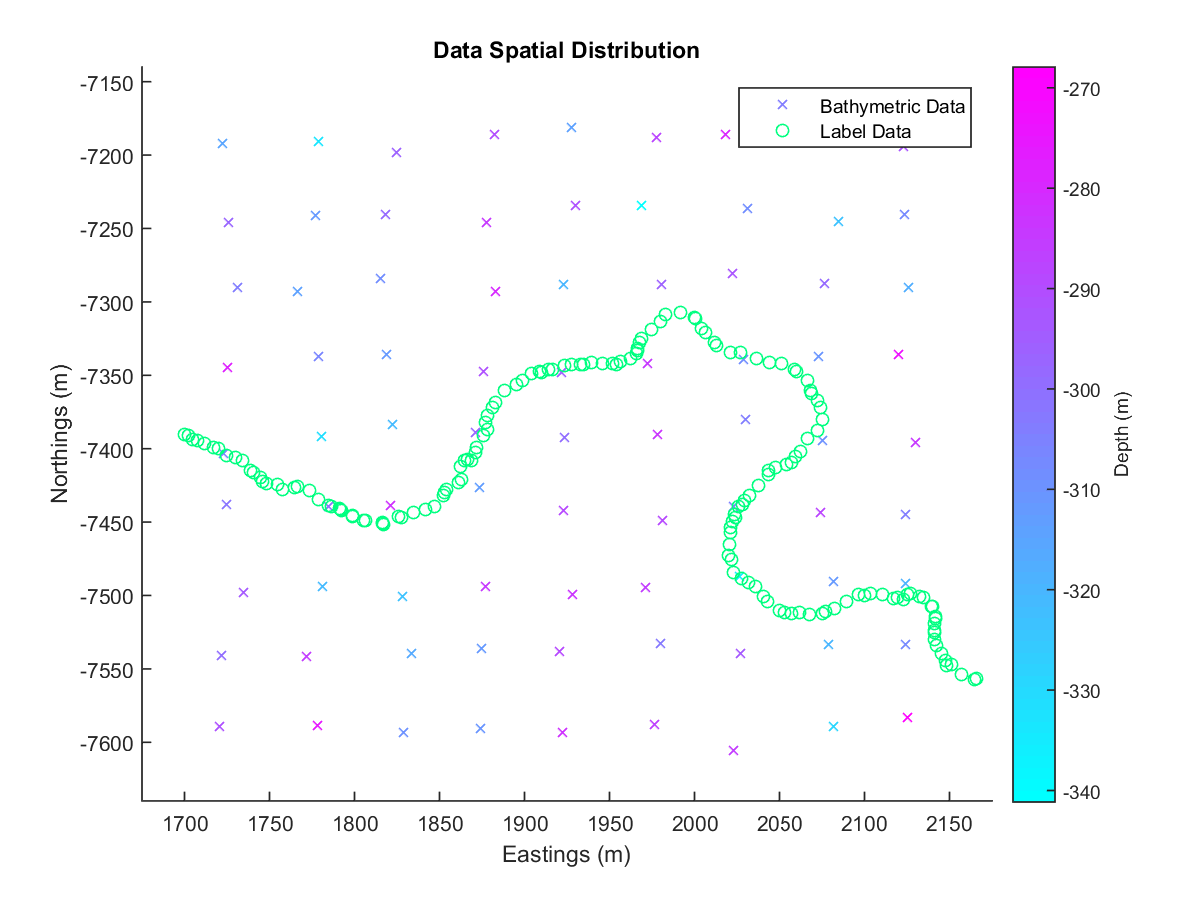
\includegraphics[width=0.9\textwidth]{Figures/illustrationBathymetricAgainstLabels.png}
				\caption{Illustration of Bathymetric and Label Data Density}
				\label{Background:OceanEnvironmentModeling:Figure:illustrationBathymetricAgainstLabels}
			\end{figure}
			
			While bathymetric data are usually collected rather uniformly, the label data are collected from past AUV missions whose trajectory are continuous curves across the ocean floor \cite{Squidle}. Due to slower AUV velocity as compared to surface ships which often employ SONAR or LIDAR techniques for bathymetry mapping, the label data are also spatially denser and concentrated on the mission trajectory, while being almost non-existent elsewhere.
			
			Therefore, in order to predict label data, the training data would need to be matched accurately. There are two straight forward choices at hand. The first is to estimate the bathymetric features at places where label data exists. However, at places near past mission paths, bathymetric data appears much more sparsely than label data, so that the feature extraction or regression prediction will yield very similar features across manly label data points. This reduces prediction power through a slow varying and limited feature group.
			
			Instead, the second choice is to estimate the label data at places where bathymetric data exists. In this setting, regions closer to past mission paths have higher volumes of label data, increasing the amount of training points. Regions further away would naturally generate more prediction uncertainty in the prediction stage.
			
			Hence, second method is chosen to be employed for data matching, in order to form our training set. Naturally, to predict environment labels from bathymetric features, we again need the Gaussian process classification model.
			
			\FloatBarrier
	
		\subsection{Feature Extraction}
		\label{Background:OceanEnvironmentModeling:FeatureExtraction}
		
			The feature extraction process assumes that the bathymetric depth data is available in grid form. That is, one can represent the available depth data $H = \{h_{k}\}_{k \in {1, 2, ..., N}}$ as $H = \{h_{ij}\}_{i \in {1, 2, ..., n_{i}}, \;\; j \in {1, 2, ..., n_{j}}}$ where varying $i$ and $j$ corresponds to varying data points in axis 1 and 2 respectively. Axis 1 and 2 is required to form an orthonormal frame. While axis 1 and 2 is usually aligned with the eastings-northings frame, it is generally not required for the feature extraction process.
			
			Without loss of generality, let $x$ and $y$ denote quantities corresponding to the orthogonal axes. We have that at $(x_{i}, y_{j})$ $(i \in {1, 2, ..., n_{i}}, \;\; j \in {1, 2, ..., n_{j}})$ the depth is measured as $h_{ij}$. The partial derivatives of various degrees of accuracy and scale can then be estimated through central differencing, as shown in \cref{Background:OceanEnvironmentModeling:Figure:centraldifferencecofficients} \cite{CentralDifferenceTable}. The author has chosen $N = 3$ neighbors for short scale slope and $N = 9$ neighbors for large scale slope.
			
			\begin{figure}[!htbp]
				\centering
					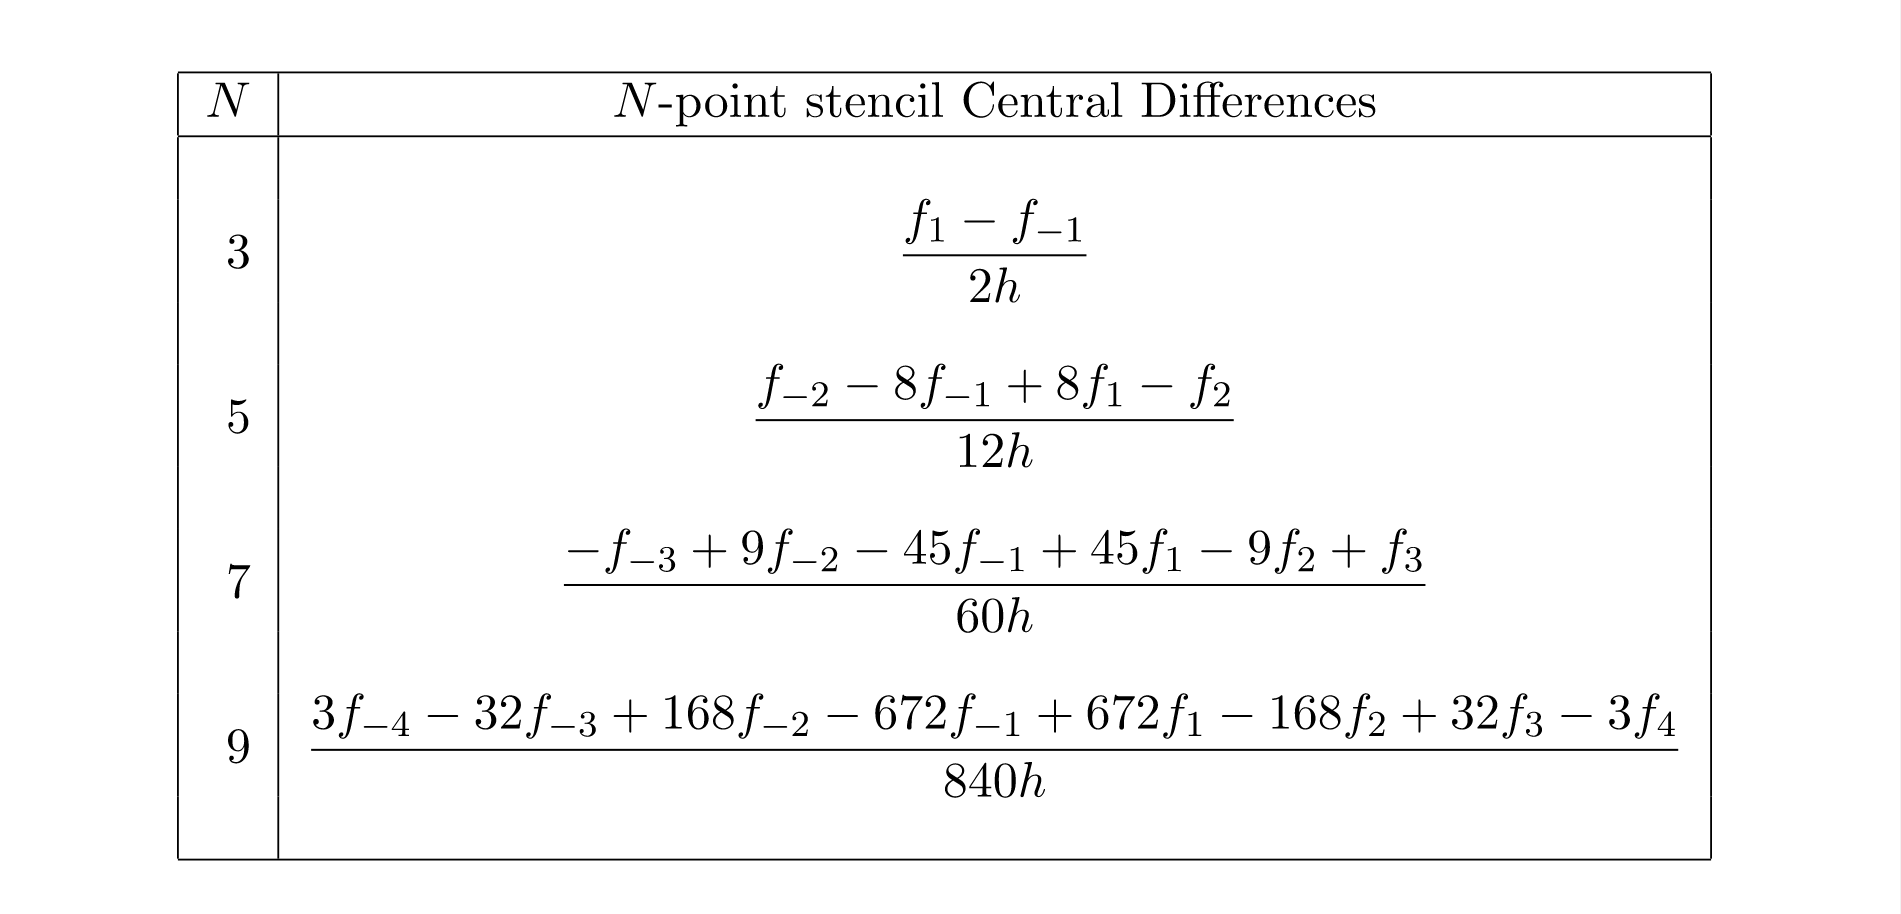
\includegraphics[width=0.9\textwidth]{Figures/centraldifferencecofficients.png}
				\caption{Finite Difference Methods: Central Difference Coefficients \\
				The subscripts $i$ represents  }
				\label{Background:OceanEnvironmentModeling:Figure:centraldifferencecofficients}
			\end{figure}			

			Central differencing is chosen as it is more numerically accurate. The disadvantages of instability and slightly higher time complexity from dynamic cases are not present in the static feature extraction process. Nevertheless, forward differencing is to be used at the boundaries of the dataset where neighboring data is missing on one side.
						
			With two axis, the result is a 2 element gradient vector. It is possible to treat the 2 elements as separate features. However, this would make the modeling problem frame dependent unnecessarily. Therefore, the magnitude of this gradient vector is taken as the slope feature. 
			
			Rugosity is a measure of local height variations in the terrain. By definition, its form is computed as $r = A_{r}/A_{g}$, the real surface area divided by the geometric surface area.
			
			Under cases without perfect grid formation, such as that shown in \cref{Background:OceanEnvironmentModeling:Figure:illustrationBathymetricAgainstLabels}, this feature extraction process becomes only an approximation. As the data set deviates from the form assumed above, it can then become necessary to estimate the features using Gaussian process regression - specifically, the multi-task Gaussian process regression. 
			
		 	On the other hand, under fine-scale bathymetric reconstructions, more sophisticated methods for deriving multi-scale measures of rugosity and slope exist. For example, under bathymetry measurements that are geo-referenced through stereo imagery, rugosity can be calculated through a Delaunay triangulated surface mesh and projecting areas onto the plane of best fit using Principal Component Analysis (PCA) \cite{StefanWilliams:Rugosity}.
							
			\FloatBarrier
				
	\section{Modeling on Test Data Sets}
	
	\section{Comparison: Laplace Approximation and Probabilistic Least Squares}
	
		Compare probability outputs, classification outputs, entropy outputs, etc
	
	\section{Comparison: OVA and AVA methods for multiclass classifiers}
	
	\section{Comparison: Probability fusion methods for multiclass classifiers}
	
%		\subsection{Normalisation Method}
%			
%		\subsection{Mode Keeping}
%			
%		\subsection{Exclusion}
			
	\section{Modeling the Scott Reef Environment}
	
		\subsection{Problems and Solutions to Big Data Analysis}
		
		\subsection{Feature Extraction}
		
		\subsection{Case with 4 Labels}
		
			(With different amounts of sampled points)
			
		\subsection{Case with 17 Labels}
		
	\section{Measuring Mutual Information}
	
		\subsection{Motivation}
			For both modeling purposes and path planning purposes, simply knowing the entropy at each query point is not enough. 
			
		\subsection{Shannon Entropy}
		
		\subsection{Lack of a Closed Form Solution}
		
	\section{A Direct Approach: Monte Carlo Sampling}
		
		\subsection{Development of Methodology}
		
			Provide pseudocode for limited and good way of doing it
			
		\subsection{Binary Classification}
		
		\subsection{Multi-class Classification}
		
	\section{A Faster Approach: Linearised Entropy}
		
		\subsection{Development of Methodology}
		
		\subsection{Binary Classification}
		
			For binary classification, linearisation is performed on the sigmoid, or response, function.
		
			The queried latent vector $\vec{f}$, a finite collection of latent function instances at query points, are distributed as a multivariate Gaussian distribution which can be computed from (equation). 
			
			\begin{equation}
				\vec{f} = [f_{1}, f_{2}, \dots, f_{n_{q}}]^{T} \sim \mathcal{N}(\vec{\mu}, \Sigma)
			\end{equation}
				
			\begin{equation}
				\pi_{i} = \sigma(f_{i}) \qquad \qquad \forall i \in I_{\mathrm{query}} = {1, 2, \dots, n_{q}}
			\end{equation}
			
		\subsection{Multi-class Classification}
		
			For multi-class classification, linearisation is performed on the softmax function for each class.
			
			Provide intuitive reason for the squashing.
			
		

\lhead{Receding Horizon Approach to Informative Path Planning}
\chapter{Receding Horizon Approach to Informative Path Planning}
\label{RecedingHorizonApproach}

	\section{Motivation}
	
		Talk about MPC and its use in control theory
		
	\section{Development of Method}
	
%		\subsection{Theory}
%		
%		\subsection{Implementation}
		
		Provide a flow diagram?
		
	\section{Properties of a Receding Horizon Solution}
	
		\subsection{Horizon Length}
		
		\subsection{Step Spacing}
		
		\subsection{Path Generation \& Natural Coordinates}
		
		\subsection{Turn Angle Limits for Smooth Paths}
		
		\subsection{Feature Space Transformations}
		
	\section{Computational Aspects}
	
		\subsection{Optimisation Process and Bottlenecks}
		
		\subsection{Relearning the Environment}
		
		\subsection{Linearised Entropy Approach}
		
		\subsection{Monte Carlo Approach}
		
	\section{Feasibility and Practicality}
	
	\section{Results with Abundant Uniform Test Data Set}
	
	\section{Results with Scarce Uniform Test Data Set}
	
	\section{Results with Simulated Track Data}
	
	\section{Results with Scott Reef Data}
	
		\subsection{Ground Truth Generation}
		
		\subsection{Practical Considerations}
		
		\subsection{Results}
		
	\section{Performance Assessment}
	
	
	


%% ----------------------------------------------------------------
% Now begin the Appendices, including them as separate files

\addtocontents{toc}{\vspace{2em}} % Add a gap in the Contents, for aesthetics

\appendix % Cue to tell LaTeX that the following 'chapters' are Appendices

\chapter{Computational Aspects of Gaussian Processes}
\lhead{Computational Aspects of Gaussian Processes}
\label{Appendix:ComputationalAspects}

	\section{Numerical Stability}
	\label{Appendix:ComputationalAspects:NumericalStability}
	
		\subsection{Cholesky Decomposition}
		\label{Appendix:ComputationalAspects:NumericalStability:Cholesky}

		\subsection{Cholesky Jittering}
		\label{Appendix:ComputationalAspects:NumericalStability:CholeskyJittering}
				
		\subsection{Solving Triangular Matrix Equations}
		\label{Appendix:ComputationalAspects:NumericalStability:SolvingTriangularMatrices}
		
		\subsection{Stable and Efficient Monte Carlo Sampling}
		\label{Appendix:ComputationalAspects:NumericalStability:MonteCarlo}
		
			Section \ref{InformativeSeafloorExploration:MCPIE} formulates the Monte Carlo prediction information entropy (MCPIE), which involves a Monte Carlo sampling stage for entropy estimation. In order to enhance the computational tractability of the approach, this thesis also investigates the practical implementation methods which would allow efficient computation for MCPIE.
			
			By definition of a GP, drawing from a GP at a \textit{finite} number of query points $X^{\star}$ is equivalent to drawing \textit{jointly} from a multivariate Gaussian distribution, as represented by \eqref{Equation:BinaryPredictiveGaussianDistribution} and \eqref{Equation:MulticlassPredictiveGaussianDistribution}. In general the sampling stage can be summarised by \eqref{Equation:GeneralMultivariateGaussianDistribution} for some mean vector $\vec{\upmu} \in \mathbb{R}^{n^{\star}}$ and covariance vector $\Sigma \in \mathbb{R}^{n^{\star} \times n^{\star}}$. 
			
			\begin{equation}
				{^{s}}\bvec{f}^{\star} \stackrel{\text{sample}}{\sim} \mathcal{N}(\vec{\upmu}^{\star}, \Sigma^{\star}) \qquad \forall s \in I_{n_{S}}
			\label{Equation:GeneralMultivariateGaussianDistribution}
			\end{equation}
			
			Note that $\stackrel{\text{sample}}{\sim}$ denotes that ${^{s}}\bvec{f}$ is not a random vector anymore but a specific vector after sampling. Instead of drawing jointly from the distribution \eqref{Equation:GeneralMultivariateGaussianDistribution} directly, a more advantageous approach involves first drawing \textit{iid} samples from the standard univariate normal distribution. That is, the samples are to be drawn independently.
			
			\begin{equation}
				\begin{aligned}
					z_{i, s} &\stackrel{\text{sample}}{\sim} \mathcal{N}(0, 1) \qquad \forall i \in I_{n^{\star}}, \forall s \in I_{n_{S}} \\
					\bvec{z}_{s} &:= \{z_{i, s}\}_{i \in I_{n^{\star}}} \in \mathbb{R}^{n^{\star}} \\
					Z &:= \{z_{i, s}\}_{i \in I_{n^{\star}}, \; s \in I_{n_{S}}} \equiv \begin{bmatrix} \bvec{z}_{1} & \bvec{z}_{2} & \dots & \bvec{z}_{n_{S}} \end{bmatrix} \in \mathbb{R}^{n^{\star} \times n_{S}}
				\end{aligned}
			\label{Equation:iidGaussianSampling}
			\end{equation}			
			
			Let $L^{\star}$ be the Cholesky Decomposition of $\Sigma^{\star}$, then $L^{\star} \bvec{z}_{s}$ incorporates the covariance structure \eqref{Equation:CovarianceInclusion}.
			
			\begin{equation}
				\begin{aligned}
					L^{\star} \bvec{z}_{s} \stackrel{\text{sample}}{\sim} \mathcal{N}(\bvec{0}, \Sigma^{\star}) \qquad \forall s \in I_{n_{S}}
				\end{aligned}
			\label{Equation:CovarianceInclusion}
			\end{equation}
			
			To incorporate the expectance $\vec{\upmu}^{\star}$, simple add it to the transformed samples \eqref{Equation:ExpectanceInclusion}.
			
			\begin{equation}
				\begin{aligned}
					\vec{\upmu}^{\star} + L^{\star} \bvec{z}_{s} \stackrel{\text{sample}}{\sim} \mathcal{N}(\vec{\upmu}^{\star}, \Sigma^{\star}) \qquad \forall s \in I_{n_{S}}
				\end{aligned}
			\label{Equation:ExpectanceInclusion}
			\end{equation}
			
			Therefore, to sample from any given multivariate Gaussian distribution $\mathcal{N}(\vec{\upmu}^{\star}, \Sigma^{\star})$, simply sample iid samples through \eqref{Equation:iidGaussianSampling} and transform the samples through \eqref{Equation:ExpectanceInclusion}, and set ${^{s}}\bvec{f}^{\star} := \vec{\upmu}^{\star} + L^{\star} \bvec{z}_{s} \quad \forall s \in I_{n_{S}}$. Generating iid samples from standard normal distributions is much faster, especially with sophisticated libraries which may have pseudo-random number generators specifically for values drawn from the standard normal distribution.
			
			Moreover, to vectorise the computation for further computational efficiency, multiple samples can be obtained at once through 
			
			\begin{equation}
				\begin{aligned}
					\begin{bmatrix} {^{1}}\bvec{f}^{\star} & {^{2}}\bvec{f}^{\star} & \dots & {^{n_{S}}}\bvec{f}^{\star} \end{bmatrix} &= \begin{bmatrix} \vec{\upmu}^{\star} + L^{\star} \bvec{z}_{1} & \vec{\upmu}^{\star} + L^{\star} \bvec{z}_{2} & \dots & \vec{\upmu}^{\star} + L^{\star} \bvec{z}_{n_{S}} \end{bmatrix} \\
					&= \mathcal{U} + L^{\star} Z \qquad \text{where} \qquad \mathcal{U} := \{\vec{\upmu}^{\star}\}^{T}_{s \in I_{n_{S}}}
				\end{aligned}
			\label{Equation:VectorisedSampling}
			\end{equation}			
			
	\section{Time Complexity}
	\label{Appendix:ComputationalAspects:TimeComplexity}
	
		Reducing computational time
		
%		\subsection{Numpy and Vectorisation}
		
		\subsection{Cholesky Update and Downdate}
		\label{Appendix:ComputationalAspects:TimeComplexity:CholeskyUpdateDowndate}
		
		\subsection{Caching learned GPs for fast prediction}
		
		\subsection{Parallelisation of GP learning and hyper-parameter batching}
		
		\subsection{Parallelisation of GP prediction and relevant subtleties}
		
%		\subsection{Fast vectorised GP drawing for regression and classification}
		
		
	\section{Time \& Spatial Complexity}
	\label{Appendix:ComputationalAspects:TimeSpaceComplexity}
	
		\subsection{Avoiding full covariance computations}
		\label{Appendix:ComputationalAspects:TimeSpaceComplexity:CovarianceAvoidance}
		
		\subsection{Taking advantage of diagonal log-likelihood Hessians}
		\label{Appendix:ComputationalAspects:TimeSpaceComplexity:DiagonalHessians}
		
		\subsection{Creating predictor objects to modularise prediction}
		
		 % Computational Aspects of Gaussian Processes
\chapter{Other Approximations for Gaussian Process Classification}
\lhead{Other Approximations for Gaussian Process Classification}
\label{Appendix:OtherApproximationsGaussianProcessClassification}

	\section{Expectation Propagation}
	
	\section{Variational Inference}
		 % Other Approximations for Gaussian Process Classification

%\input{Appendices/AppendixC} % Appendix Title

\addtocontents{toc}{\vspace{2em}}  % Add a gap in the Contents, for aesthetics
\backmatter

%% ----------------------------------------------------------------
\label{Bibliography}
\lhead{\emph{Bibliography}}  % Change the left side page header to "Bibliography"
\bibliographystyle{unsrtnat}  % Use the "unsrtnat" BibTeX style for formatting the Bibliography
\small
\bibliography{Bibliography}  % The references (bibliography) information are stored in the file named "Bibliography.bib"

\end{document}  % The End
%% ----------------------------------------------------------------